% https://pt.sharelatex.com/learn/Sections_and_chapters

\documentclass[graduacao,brazil]{ThesisPUC}
\usepackage{float}
\usepackage{enumerate}
\usepackage{listings}
\usepackage[final]{pdfpages}
\usepackage{mathtools}

%%%%%%%%%%%%%%%%%%%%%%%%%%%%%%%%%%%%%%%%%%%%%%%%%%%%%%%%%%%%%%%%%%%%%%%%%%%%%%%%

\newcommand{\Rset}{\mathbb{R}}
\newcommand{\Zset}{\mathbb{Z}}

%%%%%%%%%%%%%%%%%%%%%%%%%%%%%%%%%%%%%%%%%%%%%%%%%%%%%%%%%%%%%%%%%%%%%%%%%%%%%%%%

\autor{Julio Ribeiro da Silva}
\autorR{Ribeiro da Silva, Julio}
\orientador{S\'{e}rgio Lifschitz}
\orientadorR{Lifschitz, S\'{e}rgio}

\titulo{PrISMA}
\titulouk{PrISMA}
\subtitulo{Programa de Instru\c{c}\~{a}o \`{a} Solicita\c{c}\~{a}o de Matr\'{i}cula Acad\^{e}mica}
\dia{19} \mes{Novembro} \ano{2014}

\cidade{Rio de Janeiro}
\CDD{510}
\departamento{Inform\'atica}
\programa{Engenharia da Computa\c{c}\~{a}o}
\centro{Centro T\'{e}cnico Cient\'{i}fico}
\universidade{Pontif\'{i}cia Universidade Cat\'{o}lica do Rio de Janeiro}
\uni{PUC--Rio}
\course{Engenharia da Computa\c{c}\~{a}o}
\diploma{Bacharel em Engenharia da Computa\c{c}\~{a}o}

%%%%%%%%%%%%%%%%%%%%%%%%%%%%%%%%%%%%%%%%%%%%%%%%%%%%%%%%%%%%%%%%%%%%%%%%%%%%%%%%

  \agradecimentos{%
Primeiramente, à minha família, que esteve comigo durante todos os momentos da minha vida e tornaram possível eu chegar até aqui.

Em segundo lugar à Luiza Noronha, que foi quem esteja ao meu lado durante todo o desenvolvimento deste projeto. Assim como meu orientador Sérgio Lifschitz, a quem eu atribuo a autoria da ideia, e que também tornou a sua implantação possível.

Ao Waldecir Vicente Faria e Victor Paulo Tolini Málaga, que fizeram parte do meu grupo de Banco de Dados I, que foi onde surgiu a primeira versão do projeto. Ao João Alexandre, Diego Malone e Frederico Barnard, que também deram suas valiosas contribuições no desenvolvimento.

Ao professor Washington Braga, que foi quem apresentou o problema e sempre acreditou e defendeu o sistema, ajudando inclusive na sua divulgação para todos os alunos da PUC-Rio. E também à equipe do SAU (Sistema Acadêmico Universitário), que disponibilizou todos os dados necessários a sobrevivência do sistema.

Ao professor Luiz Fernando Bessa Seibel, que me acolheu em seu laboratório por pouco mais de três anos e sempre acreditou em mim.

À todos aqueles que estiveram ao meu lado durante toda a fase da graduação e que me ajudaram a superar os desafios, que estiveram sempre estiveram ao meu lado. Tanto as novas, quantos as velhas amizades que foram estabelecidas.

E, não menos importante, à todos os alunos da PUC-Rio que utilizaram o PrISMA. Sem vocês o projeto não teria o sucesso que foi alcançado.
}


%%%%%%%%%%%%%%%%%%%%%%%%%%%%%%%%%%%%%%%%%%%%%%%%%%%%%%%%%%%%%%%%%%%%%%%%%%%%%%%%

 \chaves{%
   \chave{Banco de dados}%
   \chave{Experi\^{e}ncia do usu\'{a}rio}%
   \chave{Aplica\c{c}\~{a}o web}%
   \chave{PrISMA}%
 }
 
 \resumo{
Na PUC-Rio, no início de cada período os alunos devem informar quais turmas gostariam de cursar no próximo período. No entanto, o número de vagas por turmas é limitado e na maior parte das vezes não é possível atender a todos os pedidos de todos os alunos. Dessa maneira, através de uma aplicação web bastante poderosa, e ao mesmo tempo de fácil uso, o PrISMA tem por objetivo auxiliar os alunos passo a passo nas suas decisões na hora de montar o seu planejamento de turmas para o período seguinte.
 }
 
 
% %%%%%%%%%%%%%%%%%%%%%%%%%%%%%%%%%%%%%%%%%%%%%%%%%%%%%%%%%%%%%%%%%%%%%%%%%%%%%%%%
 
 \chavesuk{
   \chave{Database}%
   \chave{User Experience}%
   \chave{Web application}%
   \chave{PrISMA}%
 }
 
 \resumouk{%
At PUC-Rio, in the beginning of each period students tells which classes they would like to attend. However, given that the number of vacancies for classes is limited, in most cases it is not possible to attend all requests for all students. This is the problem PrISMA aims to minimize. Thus, through a very powerful and easy to use web application, PrISMA aims to assist students step by step in their decisions when scheduling classes for the following period.
 }


%%%%%%%%%%%%%%%%%%%%%%%%%%%%%%%%%%%%%%%%%%%%%%%%%%%%%%%%%%%%%%%%%%%%%%%%%%%%%%%%

\modotabelas{fig} % nada, fig, tab ou figtab

%%%%%%%%%%%%%%%%%%%%%%%%%%%%%%%%%%%%%%%%%%%%%%%%%%%%%%%%%%%%%%%%%%%%%%%%%%%%%%%%

\begin{document}

\chapter{Introdução}

As universidades de forma geral adotam modelos muito parecidos para que alguém consiga conquistar um diploma de graduação. Para este projeto, o modelo utilizado como referência foi aquele adotado pela Pontifícia Universidade Católica do Rio de Janeiro (PUC-Rio). Todos os conceitos aqui abordados estarão condicionados neste contexto, apesar de que nada impede que possam ser estendido para as demais universidades. 

Para se cumprir um curso de graduação, disciplinas obrigatórias, eletivas e algumas outras atividades devem ser devidamente cumpridas. Como este conjunto de disciplinas é bastante extenso, e existe uma série de pré-requisitos necessários a serem cumpridos para aquelas disciplinas mais avançadas, naturalmente demora alguns anos para se conseguir o diploma. 

Portanto, define-se o conceito de período, que tem o tempo de duração da metade de um ano. Em cada período é cursado um subconjunto de disciplinas necessárias para se completar a grade do curso almejado. Para tal, antes de cada período o aluno deve se planejar quanto às disciplinas que irá cursar, horários de turmas, preferencias de professores, etc. E a proposta do PrISMA é auxiliar o aluno nesta etapa que, como será analisado, é consideravelmente crítica. 

O PrISMA é um sistema que nasceu na disciplina de Banco de Dados I no segundo período do ano de 2010, ministrada pelo meu atual orientador Sérgio Lifschitz. Desde então foram disponibilizadas duas versões para serem usadas pelos alunos da PUC-Rio, sendo a última que será abordada neste documento. 

O que esperar deste documento:

\begin{itemize}
	\item Capítulo 2: será explicado melhor o porquê do planejamento acadêmico ser complexo. 
	\item Capítulo 3: serão abordados os requisitos do sistema, na etapa de planejamento do desenvolvimento. Assim como o layout base utilizado na interface final. 
	\item Capítulo 4: será apresentada a solução final que foi implementada. Cada funcionalidade e decisão tomada será justificada. 
	\item Capítulo 5: serão apresentados os resultados atingidos pelo sistema que ficou em produção entre os anos de 2013 e 2014. 
	\item Capítulo 6: serão apresentadas outras funcionalidades que podem ser agregadas ao PrISMA, que não foi possível implementar até a data deste relatório.
	\item Anexo 1: trechos de códigos importantes utilizados no banco de dados. 
	\item Anexo 2: análise de complexidade computacional para gerar um planejamento de maneira automática.
\end{itemize}

%%%%%%%%%%%%%%%%%%%%%%%%%%%%%%%%%%%%%%%%%%%%%%%%%%%%%%%%%%%%%%%%%%%%%%%%%%%%%%%%

\chapter{Contexto} % problema a ser resolvido

A seguir serão explicados as principais dificuldades encontradas pelos alunos ao realizar seus planejamentos acadêmicos. 

Vale notar que o PrISMA foi modelado para o sistema de \textit{Solicitação de Matrícula}, não mais utilizado pela PUC-Rio. Por isso todo problema aqui citado como motivação se refere ao momento passado. No entanto, o PrISMA continua sendo útil para ser utilizado no momento presente, apoiando o sistema \textit{Matrícula em Tempo Real} durante todas as etapas.

\section{Dados descentralizados}

Para que um aluno possa fazer seu planejamento acadêmico são necessários diversos dados, são eles:

\begin{itemize}
	\item Falta-Cursar: lista de disciplinas que restam ser cursadas a fim de se obter o diploma;
	\item Micro-Horário: lista de turmas que serão disponibilizadas no próximo período, informando horários, professores, etc.;
	\item Informações das disciplinas: ementas e pré-requisitos;
\end{itemize}

A primeira dificuldade encontrada pelos alunos se refere ao acesso à esses dados apresentados. Cada um sendo apresentado em um local diferente no site da universidade, sem qualquer referencia entre eles. Com exceção do Micro-Horário que inclui o link para as informações das disciplinas.

\section{Procedimento de matrícula em 3 etapas}

A PUC-Rio organiza o procedimento de matrícula em 3 etapas, conforme segue:

\begin{enumerate}
	\item \underline{Solicitação de matrícula}: nesta etapa o aluno inicia o seu planejamento do zero, podendo solicitar qualquer turma que desejar.
	\item \underline{Ajuste}: nesta etapa o aluno poderá modificar a solicitação feita previamente, de acordo com o resultado obtido, ou mesmo caso seu planejamento tenha sido alterado.
	\item \underline{De-Para}: esta é a última etapa e, portanto, a última oportunidade para o aluno ajustar seus horários de turmas. Nesta etapa, na maior parte das vezes, restam poucas vagas nas turmas, tornando o planejamento ainda mais complicado.
\end{enumerate}

Vale ressaltar que as duas primeiras etapas são realizadas através do site da PUC-Rio, e a última de maneira presencial. 

Por motivo de falta de planejamento, uma quantidade maior do que o desejado de alunos faziam uso da terceira etapa de matrícula. Esta que, por ser presencial, exige alocação de mais recursos por parte da universidade e muitas das vezes não apresenta resultados satisfatórios, por conta da baixa quantidade de vagas restante nas turmas.

\section{Sistema fornecido pela PUC-Rio}

Abaixo será apresentado o sistema fornecido pela PUC-Rio na época que este projeto foi modelado e aquele fornecido atualmente. 

O foco principal do PrISMA está na primeira etapa de solicitação de matrícula, por isso esta que será abordada a seguir. Mas nada impede que seja utilizado para planejamento das demais etapas.

\subsection{Solicitação de Matrícula}

Este sistema era oferecido apenas na primeira etapa de solicitação de matricula. Ele se resume a uma interface para entrada de dados das turmas que serão solicitadas pelos alunos. Não tem por objetivo auxiliar o aluno no seu planejamento.

\begin{figure}[H]
    \centering
    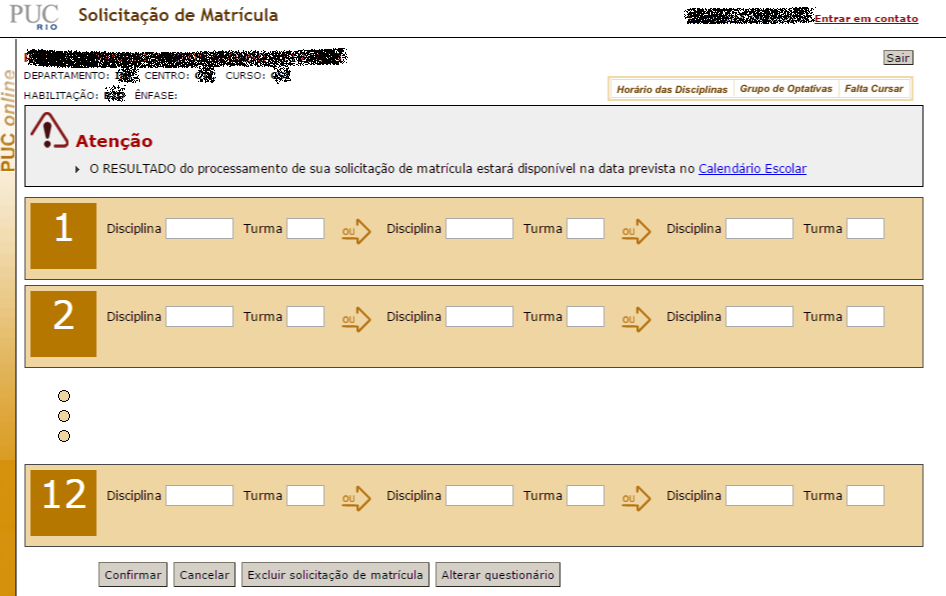
\includegraphics[width=\linewidth]{img/puc_online_antigo.png}
    \caption{Sistema Solicitação de Matrícula}
\end{figure}

Como pode ser visto na imagem acima, deve-se tomar cuidado com a ordem de preenchimento das turmas na tabela. As células presentes em uma mesma linha representam opções. E as primeiras linhas tem uma maior prioridade sobre as demais.

Ou seja, a tabela está relacionada diretamente à maneira como ela é processada, que é explicado pelo algoritmo que segue:

 \begin{enumerate}
 
 	\item Inicia procedimento na primeira linha e primeira coluna.
 	\item Verifica se não existe turma da disciplina corrente cadastrada.
 	\item Verifica se a disciplina corrente atende todos os pré-requisitos.
 	\item Verifica se o horário referente a turma solicitada ainda não está preenchido.
 	\item Verifica se ainda há vaga na turma solicitada.
 	\item Verifica se quantidade máxima de créditos não foi atingida.
 	\item Condições anteriores atendidas?
 	\begin{enumerate}
 		\item  Sim. Então matricula aluno na turma e pula para a próxima linha. 
 		\item  Não. Existe mais opção para esta linha?
 		\begin{enumerate}
 			\item Sim. Pula para a próxima opção.
 			\item Não. Pula para a próxima linha.
 		\end{enumerate}
 	\end{enumerate}
 	\item Retorna ao passo 2 e repete o processo, enquanto não alcançar o fim da tabela.
 \end{enumerate}

Como é possível perceber, por exemplo, se uma turma na primeira opção for devidamente atendida, todas aquelas que estão listadas nas próximas opções na linha corrente serão ignoradas. Um problema causado por esse comportamento acontece quando o aluno não entende corretamente o conceito de opção e coloca todas as turmas a serem solicitadas na mesma linha, mesmo quando elas não têm relação alguma. 

Outro problema se encontra na prioridade natural entre as linhas da tabela de solicitação. Por exemplo, caso na primeira linha seja escolhida a segunda opção que, por acaso, se encontra no mesmo horário da primeira opção da linha debaixo, não será possível se cadastrar nessa última por conta de horário já preenchido. 

Esse é um tipo de cascata que torna o correto preenchimento dessa tabela um grande desafio, principalmente para aqueles que não estão muito bem classificados segundo o ranking da PUC. Aqueles que estão melhor classificados não precisam nem preencher as demais opções. Basta preencher o primeiro campo de cada linha que na grande maioria das vezes não terá problemas. 

Esse sistema não é mais oferecido, mas pode-se notar que ele não tem por objetivo auxiliar o aluno no planejamento das turmas que irá solicitar. Pelo contrário, exige-se mais cuidado no seu preenchimento. 

\subsection{Matrícula em Tempo Real}

O novo sistema adotado pela PUC-Rio para solicitação das turmas por parte dos alunos representa uma grande evolução em relação ao antigo. Neste todos os dados se encontram centralizados na mesma interface e as críticas que serão apresentadas no próximo tópico são devidamente realizadas.

\begin{figure}[H]
    \centering
    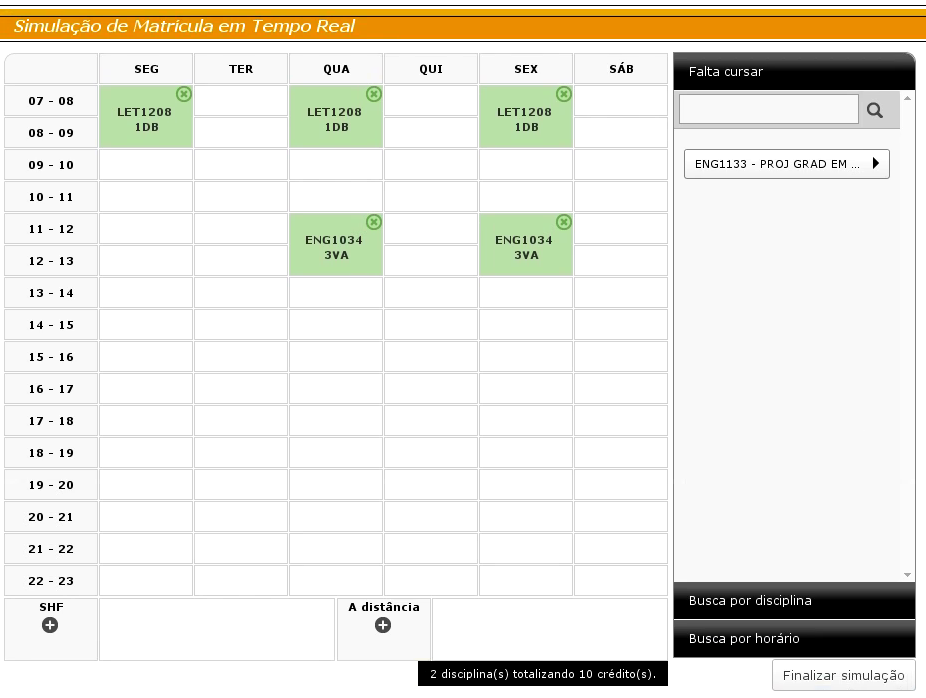
\includegraphics[width=\linewidth]{img/puc_online_novo.png}
    \caption{Matrícula em Tempo Real}
\end{figure}

Não apenas o sistema foi atualizado, como o modelo de matrícula também foi. Antes o \textit{Sistema de Solicitação de Matrícula} ficava disponível por diversos dias para todos os alunos e, após este tempo, as solicitações eram processadas respeitando a prioridade entre os alunos melhor classificados na universidade. Agora, são disponibilizados duas horas para que os alunos façam sua solicitação e que, no mesmo momento, saibam se tiveram sua solicitação atendida ou não. 

Isto é, o sistema fica disponível primeiro para os alunos melhores classificados, e assim por diante, até todos terem feito suas solicitações dentro de alguns dias. Conforme o sistema vai sendo utilizado, as turmas já serão preenchidas. Desta forma, os últimos a fazerem uso do sistema já terão uma oferta mais limitada de vagas. 

O sistema em si apresenta diversas funcionalidades semelhantes às implementadas pelo PrISMA, facilitando a etapa de solicitação. Para o planejamento, a \textit{Matrícula em Tempo Real} é oferecido para os alunos antes da etapa oficial, mas neste momento não existe planejamento quanto ao preenchimento das turmas, demais opções caso aquelas selecionadas não sejam atendidas, ou mesmo é salvo o planejamento para a etapa oficial, bastante confirmar o que havia sido feito anteriormente.

\section{Cuidados a ser tomados pelos alunos}

No decorrer do planejamento das turmas a serem solicitadas se faz necessário que os alunos estejam atentos, além das disciplinas presentes no seu Falta-Cursar, na maneira como as turmas serão combinadas e a ordem e quantidade das disciplinas que serão cursadas. Conforme será visto a seguir.

\subsection{Classificação de alunos}

Uma característica do modelo adotado pela universidade é a classificação de alunos. Essa classificação é baseada no desempenho acadêmico do aluno e na quantidade de créditos totais cumpridos. Cada disciplina contém uma quantidade de créditos associada, portanto este último se refere à quantidade de disciplinas e o quão perto está de cumprir o curso. 

Essa informação é utilizada para priorizar os alunos na hora de serem matriculados nas turmas. Tendo maior prioridade aqueles melhor classificados.  

Dessa forma, dado que a quantidade de vagas nas turmas é limitada, aqueles alunos pior classificados terão sua gama de escolhas reduzida. Por esse motivo seus planejamentos se mais complicados. Além de escolher a turma, deve-se pensar nas demais possibilidades caso aquela solicitação não seja atendida.

\subsection{Conflitos de horários}

Uma das regras que devem ser obedecidas ao se solicitar uma turma é a seguinte: não é permitido ao aluno se matricular em duas turmas que estejam alocadas no mesmo horário. 

Levando em consideração o sistema \textit{Solicitação de Matrícula} disponibilizado pela PUC-Rio, que tem uma maneira particular de lidar com as demais opções, e a classificação de alunos, limitando assim a gama de escolhas, mais cuidado deve ser tomado na etapa de planejamento.

\subsection{Pré-requisitos}

Pré-requisitos são restrições necessárias à algumas disciplinas que tenham necessidade de que o aluno tenha algum conhecimento prévio para cursá-la. Por isso, ao solicitar uma turma de determinada disciplina, deve-se tomar o cuidado de avaliar se é possível mesmo cursá-la. 

Caso seja feita a solicitação de alguma disciplina que não tenham os pré-requisitos atendidos, ela apenas será negada e o planejamento realizado previamente já terá sido modificado.

\section{Restrições}

Outras restrições restrições de matrícula que deve-se tomar cuidado:

\begin{itemize}
	\item \underline{Lei do Básico}\footnote{http://www.puc-rio.br/sobrepuc/depto/dar/procedimentos.html\#limitada\_cb-ctc}: os alunos de engenharia devem cursar um conjunto de disciplinas que pertencem ao chamado Ciclo Básico. Caso estas não sejam cumpridas dentro de sete períodos, o aluno só poderá cursar estas pendentes e uma de fora.
	\item \underline{Quarta ou quinta tentativa}\footnote{http://www.puc-rio.br/sobrepuc/depto/dar/procedimentos.html\#limitada}: caso o aluno vá cursar alguma disciplina pela quarta ou quinta vez, ele só pode se matricular no máximo em quatro disciplinas no próximo período.
\end{itemize}


\chapter{Modelagem}

De acordo com o contexto apresentado no capítulo anterior, propõe-se o PrISMA. Uma ferramenta web para apoio aos alunos da PUC-Rio, que tem por objetivo centralizar todos os dados necessários, oferecer ferramentas de apoio e facilitar a visualização dos dados referentes ao planejamento acadêmico. 

Visando formalizar as funcionalidades desejadas para auxiliar os alunos, definimos os requisitos funcionais abaixo:

\begin{itemize}
	\item Centralização dos dados
	\begin{itemize}
		\item Micro Horário 
		\item Falta Cursar 
		\item Ementa e pré-requisito das disciplinas 
	\end{itemize}
	\item Processamento de pré-requisitos 
	\item Fácil visualização e combinação das turmas 
	\item Acesso de qualquer lugar 
	\item Visualização de críticas 
	\begin{itemize}
		\item Micro Horário 
		\item Conflitos de horários 
		\item Quantidade máxima de créditos 
		\item Demais regras restritivas (capítulo 2.5) 
	\end{itemize}
	\item Estatísticas
\end{itemize}

E visando a redução dos custos, qualidade e confiabilidade do serviço a ser fornecido, definimos os requisitos não funcionais:


\begin{itemize}
	\item Controle de acesso 
	\item Minimizar carga no servidor 
	\begin{itemize}
		\item Tráfego de dados 
		\item Processamento 
		\item Armazenamento 
	\end{itemize}
	\item Código de fácil manutenção
\end{itemize}

Esses requisitos também são resultado das versões que antecederam esta que está sendo documentada. A primeira versão do PrISMA foi desenvolvida no segundo período para a disciplina de Banco de Dados I, ministrada pelo professor Sérgio Lifschitz. Uma versão pouco modificada foi disponibilizada aos alunos nos anos de 2011 e 2012.  

A última versão foi modelada e implementada no final do ano de 2012. Nesta época, um grupo do curso de Design, da PUC-Rio, composto por Gabriel Martinelli, Denis Neves, Glauber Borges e Maurício Fragale, havia trabalhado em cima do mesmo contexto e apresentou a seguinte solução:

\begin{figure}[H]
    \centering
    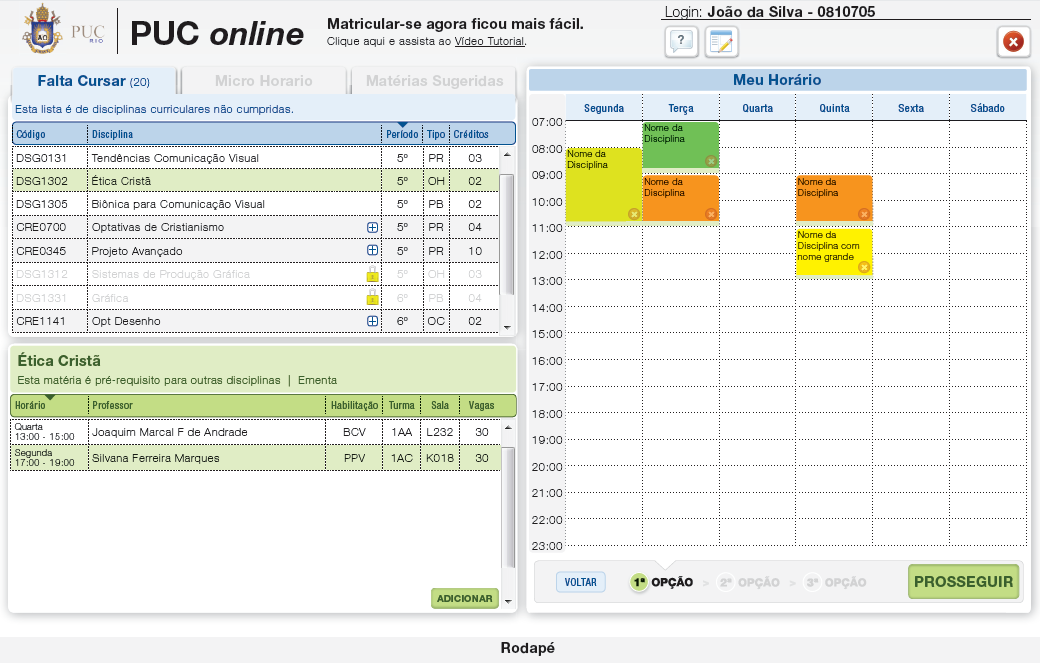
\includegraphics[width=\linewidth]{img/designer.png}
    \caption{Versão proposta pelos designers}
\end{figure}

Segundo os requisitos funcionais de centralização de dados e fácil visualização do planejamento, a solução acima atende satisfatoriamente as necessidades dos alunos. 

No lado direito da interface é apresentada uma tabela de horários semanal, que apresenta cada turma selecionada em cima do seu respectivo horário, segundo o planejamento. Já no lado esquerdo são apresentadas as disciplinas do Falta-Cursar, Micro-Horário e disciplinas sugeridas. Sendo esta última fora do escopo, sendo assim substituída pelas disciplinas selecionadas, no mesmo formato apresentado pelo sistema Solicitação de Matrícula, da PUC-Rio.

\begin{figure}[H]
    \centering
    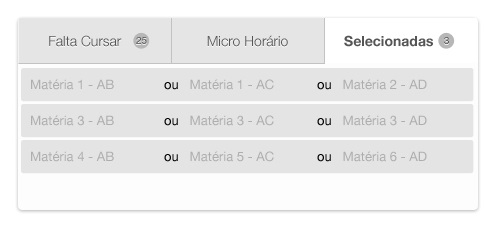
\includegraphics[width=0.8\linewidth]{img/selecionadas.jpg}
    \caption{Aba de disciplinas selecionadas}
\end{figure}

No próximo capítulo será apresentada a etapa de modelagem, assim como todas as ferramentas e decisões tomadas para que todos os requisitos sejam atendidos. No capítulo 4 será apresentada a solução final, que utilizou este conceito como base.

\chapter{Implementação}

Neste capítulo serão abordados os aspectos técnicos da última versão implementada do PrISMA, assim como as decisões quanto às ferramentas e aos padrões que foram adotados. As versões mais antigas não serão abordadas por terem sido implementadas sem grandes preocupações com a Engenharia de Software em si, se tratando apenas de uma etapa introdutória ao mundo do desenvolvimento Web.

A solução é baseada em uma aplicação Web. Isto é, existe um servidor com o objetivo de persistir e compilar os dados que serão apresentados aos usuários, e apenas os seus dados. E existe uma aplicação que é executada no navegador dos usuários, que utiliza extensivamente de requisições dinâmicas de forma que seja reduzido ao máximo o tráfego de dados, consequentemente a carga no servidor, e as transições dentro da aplicação fiquem mais suaves a ponto de se aproximem de uma aplicação desktop.

O servidor utilizado para hospedar o projeto foi disponibilizado pelo Sérgio Lifschitz que, com a ajuda do suporte do Departamento de Informática (principalmente o Anderson Oliveira da Silva), foi relacionado com o domínio “prisma.inf.puc-rio.br”. A configuração utilizada no servidor foi a distribuição TurnKey Linux, com servidor Apache\cite{Apache}, servidor PostgreSQL\cite{PostgreSQL} e pacotes para que seja possível a execução de scripts em PHP\cite{PHP}. Na configuração final fez-se uso de SSL, sem a disponibilidade de certificado verificado por Autoridade Certificadora.

Todo código gerado foi versionado utilizando-se GIT e hospedado na plataforma GitHub\footnote{https://github.com/PrismaDev/prisma}. Sendo open-source, todos podem contribuir, usar como referência ou mesmo reutilizar todo o projeto.

O padrão MVC (Model-view-controller) foi utilizado duas vezes na implementação do sistema. A primeira no lado do servidor (back-end), outra no lado do aplicativo que é executado no navegador (front-end). A comunicação entre essas duas camadas se dá por intermédio dos respectivos controllers, utilizando requisições dinâmicas e o formato JSON para transmissão dos dados.

\section{Banco de Dados}

Nas primeiras versões foi utilizado o SGBD MySQL para persistência e consistência dos dados. Na última versão, o PostgreSQL. A mudança foi realizada por conta do último ter melhor desempenho, ser mais rico em funcionalidades, ser mais seguro e ter a preferência dos desenvolvedores.

Abaixo será explicado todo o modelo desenvolvido, assim como as decisões tomadas.

\subsection{Tabelas}

Utilizando a ferramenta DbVisualizer\cite{DbVisualizer} foi gerado o esquema relacional do banco de dados implementado para o PrISMA.

\begin{figure}[H]
    \centering
    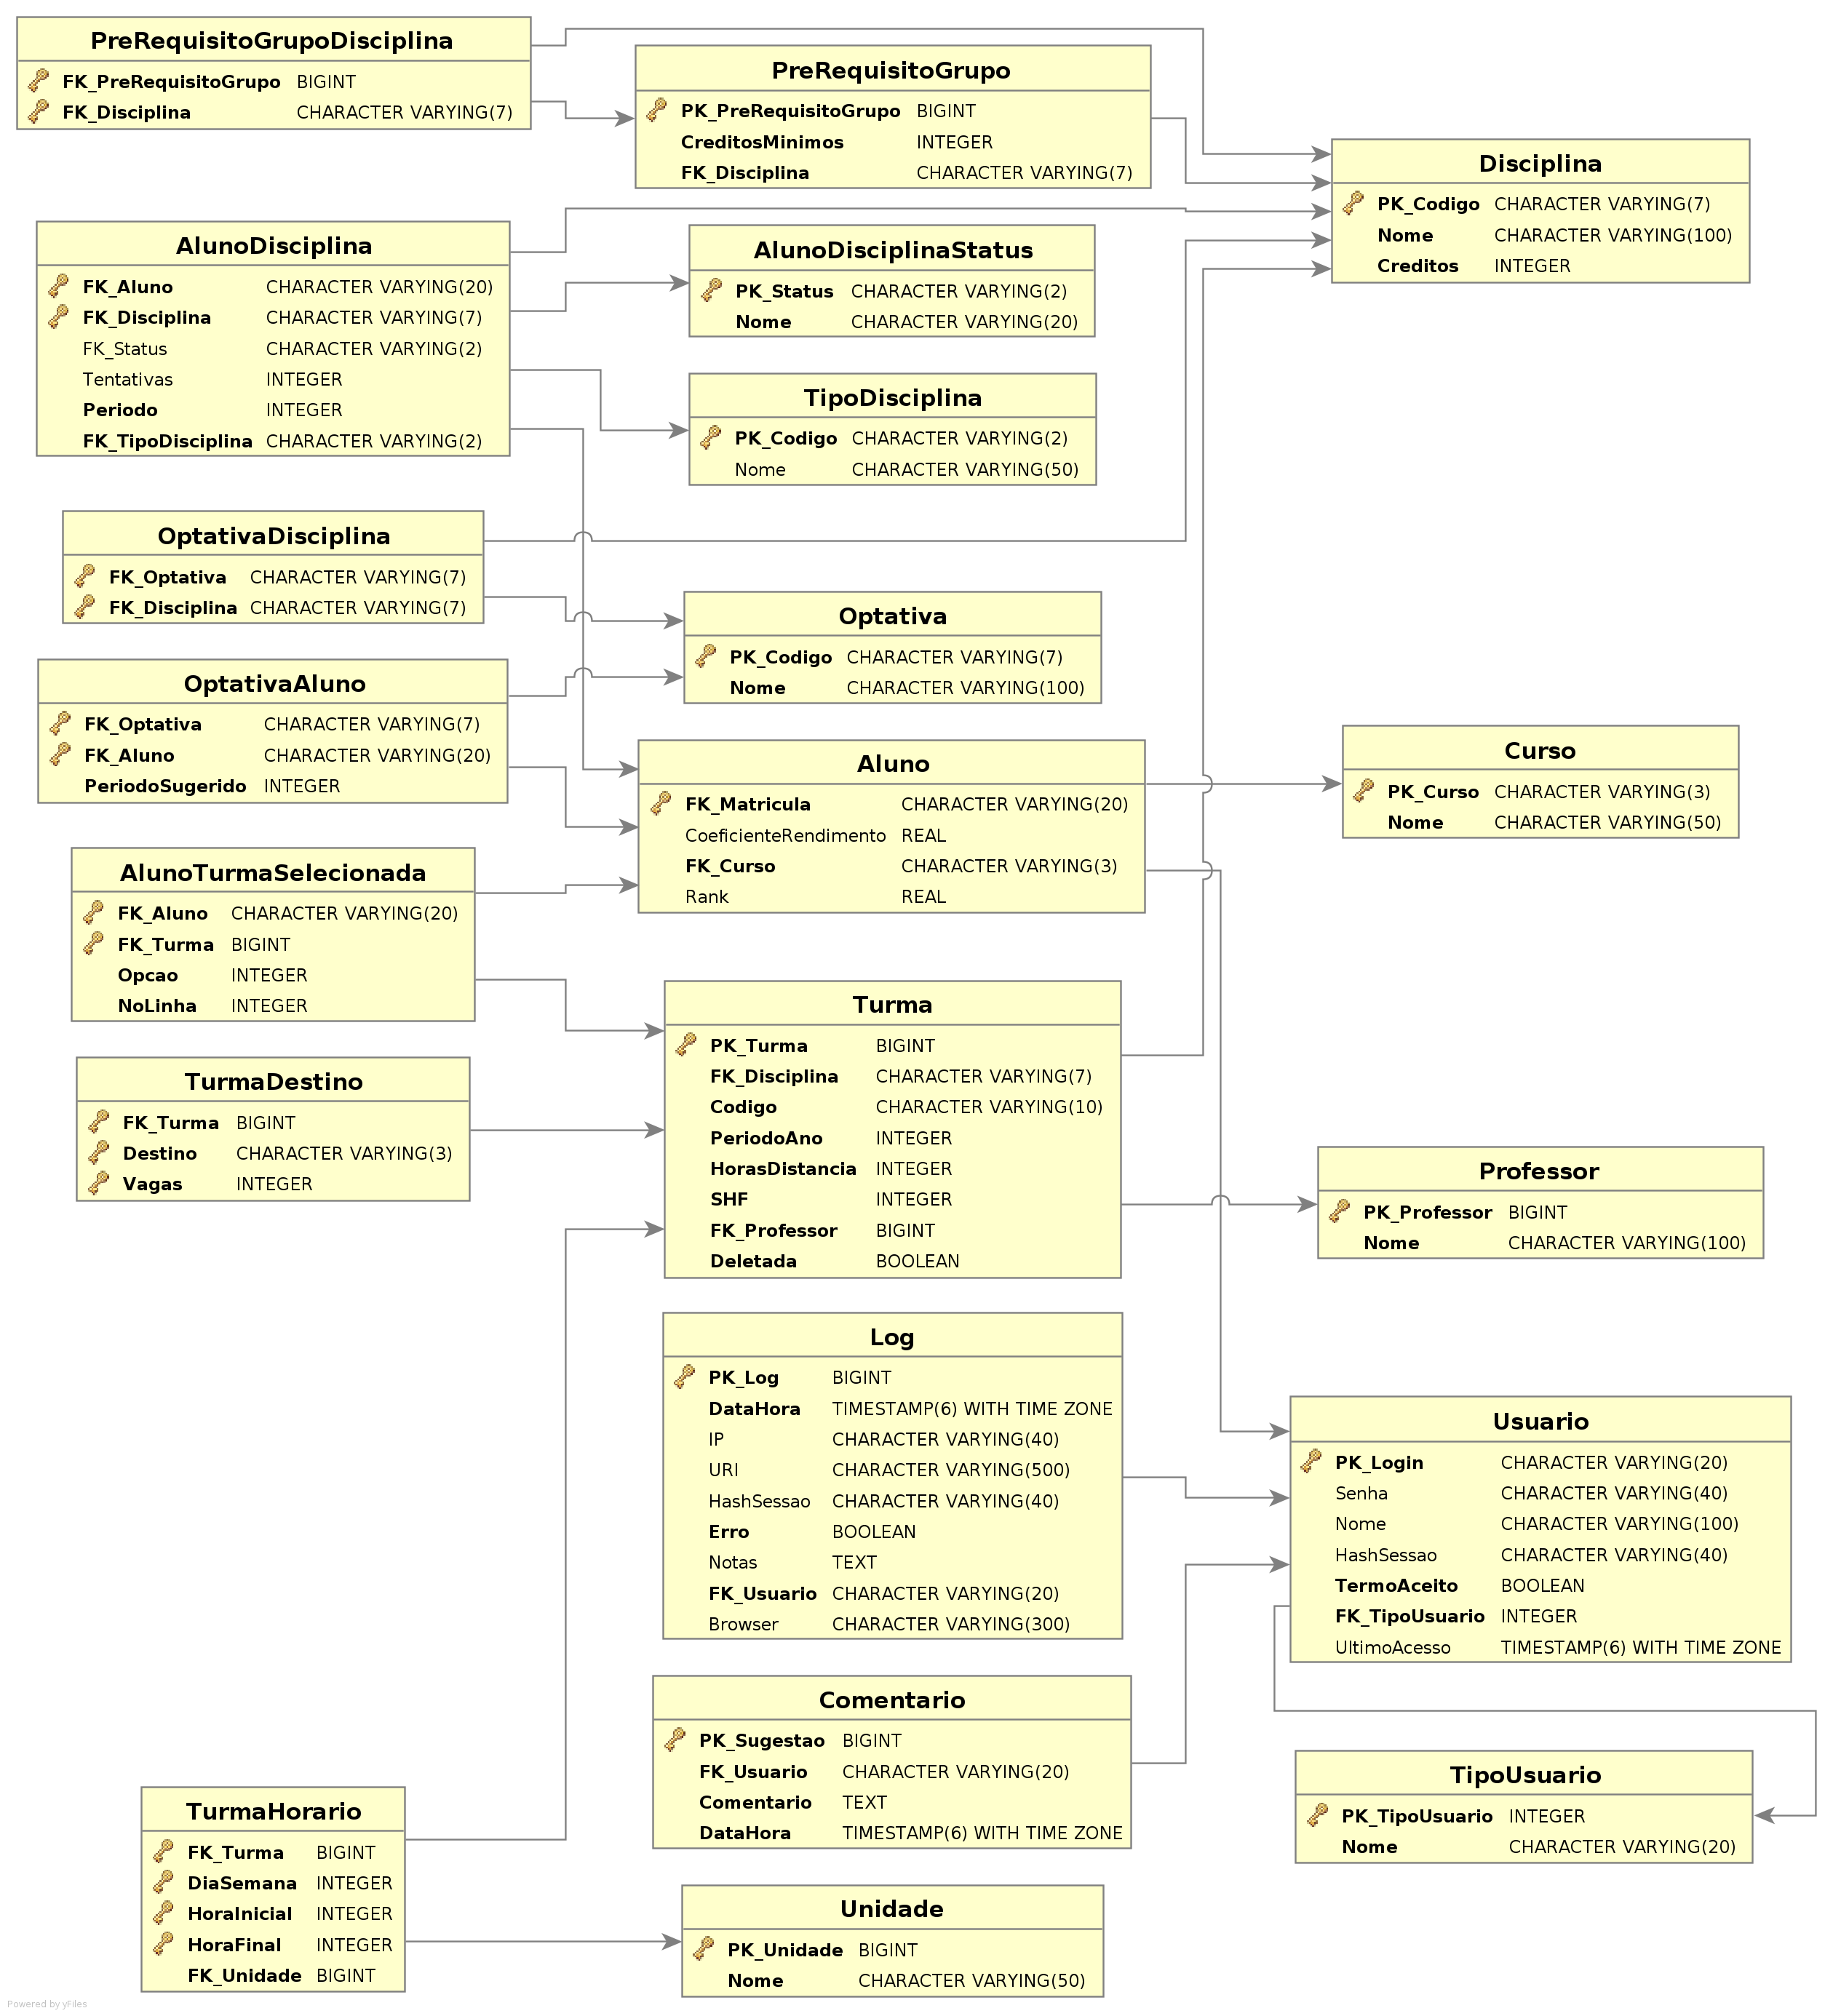
\includegraphics[width=0.98\linewidth]{img/dbvisualizer.png}
    \caption{Esquema Relacional do Banco de Dados}
\end{figure}

Com base no esquema acima, segue a descrição de cada tabela:

\begin{itemize}

	\item \underline{Aluno}: é um tipo de Usuário no sistema, no caso, aquele que realizará a escolha de Turmas para montar sua grade;
	\begin{itemize}
		\item FK\_Matrícula: referência login do Usuário que, quando Aluno, é a sua matrícula;
		\item CoeficienteRendimento: coeficiente de rendimento do aluno acumulado;
		\item FK\_Curso: referência para o curso do aluno;
		\item Rank: valor utilizado para classificar alunos de acordo com sua prioridade na hora de fazer suas escolhas.
	\end{itemize}

	\item \underline{AlunoDisciplina}: representa o relacionamento de um Aluno com Disciplina;
	\begin{itemize}
		\item FK\_Aluno: referência para Aluno;
		\item FK\_Disciplina: referência para disciplina;
		\item FK\_Status: referência para AlunoDisciplinaStatus;
		\item Tentativas: quantidade de vezes que aluno tentou cursar uma turma desta disciplina;
		\item Periodo: Caso a disciplina tenha sido cursada alguma vez, se trata do período que foi cursada pela última vez. Caso contrário, se trata do período sugerido para ser cursada, caso obrigatória;
		\item FK\_TipoDisciplina: referência para TipoDisciplina;
	\end{itemize}

	\item \underline{AlunoDisciplinaStatus}: tabela estática que explicita quais Status são possíveis para o relacionamento entre Aluno e Disciplina. Possui as tuplas (CP, cumpriu), (EA, em andamento) e (NC, não cumpriu);
	\begin{itemize}
		\item PK\_Status: identificador único
		\item Nome: descrição do Status;
	\end{itemize}

	\item \underline{AlunoTurmaSelecionada}: relaciona Aluno com Turma, representando as escolhas feitas pelos alunos;
	\begin{itemize}
		\item FK\_Aluno: referência para o Aluno;
		\item FK\_Turma: referência para a Turma;
		\item Opcao: opção referente à tabela de entrada de dados, no modelo antigo do PUC Online;
		\item NoLinha: número da linha referente à tabela de entrada de dados, no modelo antigo do PUC Online;
	\end{itemize}

	\item \underline{Comentário}: armazena as sugestões feitas pelos Usuários;
	\begin{itemize}
		\item PK\_Sugestão: identificador único gerado automaticamente;
		\item FK\_Usuario: referência para o Usuário que fez a sugestão;
		\item Comentário: texto que representa o comentário em si;
		\item DataHora: data e hora que o comentário foi feito;
	\end{itemize}

	\item \underline{Curso}: registra os diferentes Cursos de graduação que podem ser cursados pelos Alunos;
	\begin{itemize}
		\item PK\_Curso: identificador único;
		\item Nome: nome do curso;
	\end{itemize}

	\item \underline{Disciplina}: representa uma Disciplina;
	\begin{itemize}
		\item PK\_Codigo: identificador único composto por 3 letras e 4 números;
		\item Nome: nome da disciplina;
		\item Creditos: quantidade de créditos que o aluno acumulará ao cumprir a disciplina;
	\end{itemize}

	\item \underline{Log}: registra toda interação feita pelo Usuário;
	\begin{itemize}
		\item PK\_Log: identificador único gerado automaticamente;
		\item DataHora: data e hora do registro;
		\item IP: endereço IP do usuário que gerou o log;
		\item URI: endereço relacionado à requisição feita pelo usuário;
		\item HashSessao: identificador da sessão do usuário;
		\item Erro: indica se foi registrado algum erro no processamento da requisição;
		\item Notas: texto detalhando o erro ou anormalidade constatada;
		\item FK\_Usuario: referência ao Usuário;
		\item Browser: informa qual navegador foi utilizado ao efetuar a requisição;
	\end{itemize}

	\item \underline{Optativa}: representa um grupo de Optativas (obrigatoriedade de cursar ao menos uma Disciplina pertencente ao grupo);
	\begin{itemize}
		\item PK\_Codigo: identificador do grupo de optativa, composto por 3 letras e 4 números;
		\item Nome: nome do grupo de optativa;
	\end{itemize}

	\item \underline{OptativaAluno}: parte do Falta-Cursar, onde é definido quais Optativas os Alunos devem cursar;
	\begin{itemize}
		\item FK\_Optativa: referência para Optativa;
		\item FK\_Aluno: referência para Aluno;
		\item PeriodoSugerido: período sugerido para que seja cursada pelo Aluno;
	\end{itemize}

	\item \underline{OptativaDisciplina}: relaciona Optativa com Disciplina, informando quais Disciplinas compõem o grupo de Optativas;
	\begin{itemize}
		\item FK\_Optativa: referência para Optativa;
		\item FK\_Disciplina: referência para Disciplina;
		\item FK\_Optativa: referência para Optativa;
	\end{itemize}

	\item \underline{PreRequisitoGrupo}: cada disciplina pode ter mais de um grupo de Pré-Requisito relacionado. Para que o Pré-Requisito para uma Disciplina seja validado, apenas um grupo precisa ser atendido. Isto é, todas as Disciplinas do grupo sejam cursadas e a quantidade mínima de créditos atendida;
	\begin{itemize}
		\item PK\_PreRequisitoGrupo: identificador único gerado automaticamente;
		\item CreditosMinimos: quantidade mínima de créditos acumulados pelos Alunos para que este grupo seja atendido;
		\item FK\_Disciplina: referência para a Disciplina que possui este pré-requisito;
	\end{itemize}

	\item \underline{PreRequisitoGrupoDisciplina}: disciplinas que compõem um grupo de Pré-Requisito. Todas devem ser cursadas para que o grupo de Pré-Requisito seja atendido;
	\begin{itemize}
		\item FK\_PreRequisitoGrupo: referência para PreRequisitoGrupo;
		\item FK\_Disciplina: referência para disciplina que faz parte do grupo;
	\end{itemize}

	\item \underline{Professor}: representa os professores;
	\begin{itemize}
		\item PK\_Professor: identificador único gerado automaticamente;
		\item Nome: nome do professor;
	\end{itemize}

	\item \underline{TipoDisciplina}: tabela estática que informa se Disciplina do Falta-Cursar é eletiva, optativa, obrigatória, etc.;
	\begin{itemize}
		\item PK\_Codigo: identificador único;
		\item Nome: descrição;
	\end{itemize}

	\item \underline{TipoUsuário}: tabela estática que informa qual o tipo de Usuário. Pode ser administrador, aluno, etc.;
	\begin{itemize}
		\item PK\_TipoUsuario: identificador único;
		\item Nome: descrição;
	\end{itemize}

	\item \underline{Turma}: representa uma Turma. Deve, obrigatoriamente, ter um Professor relacionado;
	\begin{itemize}
		\item PK\_Turma: identificador único gerado automaticamente;
		\item FK\_Disciplina: referência à Disciplina correspondente;
		\item Codigo: código composto por 3 caracteres alfanuméricos, que identificam a turma para cada disciplina;
		\item PeriodoAno: período e ano que a turma está sendo oferecida;
		\item HorasDistancia: quantidade de horas semanais que a turma exige que seja cumprida a distância (sem sala de aula);
		\item SHF: sem horário fixo;
		\item FK\_Professor: referência para o Professor relacionado;
		\item Deletada: booleano que invalida Turma;
	\end{itemize}

	\item \underline{TurmaDestino}: a quantidade de vagas de uma Turma pode ser reservada para diferentes Cursos;
	\begin{itemize}
		\item FK\_Turma: referência para Turma;
		\item Destino: código do Destino (Destino não modelado, este código é apenas exibido para o aluno);
		\item Vagas: quantidade de vagas reservadas ao destino relacionado;
	\end{itemize}

	\item \underline{TurmaHorario}: relaciona as Turmas com seus respectivos horários de aula;
	\begin{itemize}
		\item FK\_Turma: referência para Turma;
		\item DiaSemana: inteiro identificando o dia da semana;
		\item HoraInicial: inteiro identificando hora de início da aula;
		\item HoraFinal: inteiro identificando hora de término da aula;
		\item FK\_Unidade: campus da universidade onde a turma é ministrada;
	\end{itemize}

	\item \underline{Unidade}: representa diferentes campus da universidade;
	\begin{itemize}
		\item PK\_Unidade: identificador único gerado automaticamente;
		\item Nome: nome do local onde fica localizado o campus;
	\end{itemize}

	\item \underline{Usuário}: representa um Usuário;
	\begin{itemize}
		\item PK\_Login: representa o login do usuário no sistema;
		\item Senha: MD5 da senha do usuário;
		\item Nome: nome do usuário;
		\item HashSessao: identificador único de sessão do usuário. É atualizado a cada novo login. É necessário para efeito para o log;
		\item TermoAceito: variável booleana que indica aceitação do termo de compromisso para utilização do sistema. Caso não seja aceito, o acesso não é concedido.
		\item FK\_TipoUsuario: define se usuário é Aluno, Administrador, etc.;
		\item UltimoAcesso: data e hora do último login do usuário;
	\end{itemize}

\end{itemize}

\subsection{Visões}

As visões, nesta implementação, abstraem as consultas mais complexas da camada da aplicação. São elas:

\begin{itemize}
	\item \underline{AlunoDisciplinaTurmaSelecionada}: para cada disciplina selecionada para o aluno, também retorna a quantidade total de vagas e a quantidade de alunos que também selecionaram esta Turma, mas que tem classificação superior ao Aluno corrente no ranking da PUC-Rio. Não inclui turmas que tenham sido deletadas;
	\item \underline{EstatisticaDemandaHorario}: para cada horário, conta-se a quantidade de alunos que tenham escolhido uma turma neste respectivo horário;
	\item \underline{EstatisticaDemandaTurma}: conta quantos alunos escolheram determinada Turma. Informa também a quantidade de vagas disponível;
	\item \underline{FaltaCursarOptativa}: retorna apenas as optativas que fazem parte do Falta-Cursar. Isto é, que ainda não tenham sido cumpridas;
	\item \underline{FaltaCursarOptativaDisciplina}: para as optativas que fazem parte do Falta-Cursar, informa as disciplinas que compõem o grupo e a situação dos Alunos frente a elas. Isto é, se estão cursando e/ou se estão aptos a cursá-las;
	\item \underline{LogAcessoSegundo}: estatística de acesso ao sistema, por segundo. Conta cada requisição realizada pelos Usuários;
	\item \underline{LogAlunoAno}: estatística que informa a quantidade de alunos que acessaram o sistema, agrupado pelo ano de entrada na universidade;
	\item \underline{LogAlunoCurso}: estatística quanto ao percentual de alunos que acessaram o sistema, por curso. Isto é, informa qual é a quantidade total de alunos por curso e a quantidade que efetivamente fez uso do sistema;
	\item \underline{LogAlunoSelecionada}: estatística que informa a quantidade de alunos que selecionaram ao menos uma Turma e a quantidade média de turmas selecionadas por eles. Se trata apenas de uma tupla;
	\item \underline{LogErro}: se trata apenas da tabela de log filtrada pelo atributo Erro, que indica quando ocorreu algum erro inesperado;
	\item \underline{LogHistogramaBrowserUsuario}: estatística que informa quantos usuários utilizaram os diferentes navegadores existentes;
	\item \underline{LogQuantidadeUsuario}: estatística que informa a quantidade de usuários que acessaram o sistema ao menos uma vez;
	\item \underline{LogUsuarioAcesso}: conta quantas vezes cada usuario acessou o sistema e, utilizando esse valor, agrupa-se os usuarios que acessaram a mesma quantidade de vezes e realiza a contagem, para cada quantidade de acesso;
	\item \underline{LogUsuarioDia}: quantidades de usuários únicos que acessaram o sistema, por dia;
	\item \underline{MicroHorario}: recupera o Micro-Horário original, realizando a união das tabelas Disciplinas, Turmas, Professor, TurmaHorario e TurmaDestino;
	\item \underline{MicroHorarioDisciplina}: para cada Aluno e para cada Disciplina, informa se já foi cursada e/ou está apta a ser cursada;
	\item \underline{TurmaHorarioUnidade}: união entre TurmaHorario e TurmaUnidade apenas;
	\item \underline{TurmaProfessor}: união entre Turma e Professor apenas;
	\item \underline{UsuarioAluno}: relacionamento entre Usuario e Aluno apenas;
\end{itemize}

\subsection{Funções}

As funções abstraem consultas que são realizadas por diferentes visões, ou mesmo outras funções, ou que são mais complexas que as demais. São elas:

\begin{itemize}
	\item \underline{AlunoCreditos( $<$MatriculaAluno$>$, $<$StatusSituacao$>$ )}: conta a quantidade de créditos composto pelas disciplinas tenham a situação passada por parâmetro, para um determinado Aluno. Caso a situação seja NC (não cumpriu), considera-se apenas as disciplinas do Falta-Cursar;
	\item \underline{AlunoCreditosCursados( $<$MatriculaAluno$>$ )}: análoga à função anterior, só que apenas para disciplinas que tenham status CP (cumpriu);
	\item \underline{AlunoDisciplinaApto( $<$MatriculaAluno$>$, $<$CodigoDisciplina$>$ )}: para este par Aluno-Disciplina, verifica-se se ele atende todos os pré-requisitos para cursar a dada disciplina. Caso retorno seja 2, pode cursar. Caso 1, cuidado, disciplina está sendo cursada ou quantidade de créditos necessário para cursá-la depende das suas aprovações no período corrente. Caso 0, presa por pré-requisito. Para cada par Aluno-Disciplina, verifica-se se há algum grupo de pré-requisito que seja composto apenas por disciplinas que já tenham sido cumpridas;
	\item \underline{AlunoDisciplinaSituacao( $<$MatriculaAluno$>$, $<$CodigoDisciplina$>$ )}: para cada Aluno e Disciplina, informa situação. Isto é, se foi cumprida, se está em andamento ou se não foi cumprida;
	\item \underline{AlunoOptativaCursada( $<$MatriculaAluno$>$, $<$CodigoOptativa$>$ )}: para cada Optativa que deve ser cursada pelo Aluno, verifica-se se há pelo menos uma Disciplina deste grupo que tenha sido cumprida pelo Aluno;
	\item \underline{AlunoTurmaRank( $<$MatriculaAluno$>$, $<$IdTurma$>$ )}: para cada Turma selecionada por um Aluno, conta quantos alunos que também selecionaram aquela Turma tem classificação maior do que o Aluno referenciado;
	\item \underline{DisciplinaTemPrequisito( $<$CodigoDisciplina$>$ )}: apenas informa se existe referência à dada disciplina na tabela PreRequisitoGrupo;
	\item \underline{LimpaBanco()}: limpa banco de dados, sem zerar tabelas estáticas;
	\item \underline{TurmaVagasTotal( $<$IdTurma$>$ )}: para a dada Turma, informa a quantidade de vagas total que está sendo oferecida;
\end{itemize}


\section{Aplicação do servidor}

As requisições efetuadas por cada cliente são direcionadas ao servidor para uma porta e um IP específico. Esta porta deve ter sido previamente aberta por um servidor HTTP, que estará esperando as conexões dos clientes. Esse servidor, por sua vez, deve encaminhar as requisições para a aplicação para que sejam devidamente respondidas.

A aplicação, neste caso, foi escrita em PHP. Para auxiliar no seu desenvolvimento foi utilizado o framework Very Simple PHP Rest Framework\cite{RestFW}, conforme será explicado a seguir.

\subsection{Alternativas e escolhas}

\paragraph{Servidor HTTP}

Diversos outros servidores HTTP estão disponíveis, no entanto nenhum é tão utilizado e reconhecido quanto o da Apache. Este se demonstra muito fácil de ser configurado e já vem instalado em grande parte das distribuições Linux. Dado que qualquer outra escolha atenderia as necessidades do sistema da mesma maneira, este foi escolhido por ser mais conveniente.

\paragraph{Linguagem da aplicação}

A linguagem PHP tem uma grande vantagem de ter uma curva de aprendizado muito suave, principalmente pra quem já sabe programar em outras linguagens como Java e C. Dessa forma, por conta de maior domínio dos programadores, e pelo fato do projeto não exigir nenhuma operação muito complexa que precisasse ser otimizada, por conveniência foi escolhido o PHP mesmo.

\paragraph{Framework}

Diversos frameworks estão disponíveis em PHP. Dentre eles: Zend Framework, Symfony, CakePHP, etc. No entanto, todos apresentam muitas funcionalidades e cada um tem a sua forma de lidar com a organização do projeto em si.

Por conta disso foi desenvolvido o Very Simple PHP Rest Framework\cite{RestFW}, que se trata de um framework bastante minimalista, que lida apenas com o correto direcionamento das requisições para os devidos controles, controla a conexão com o banco de dados e lida com o processamento de templates que serão entregues ao navegador.


\subsection{Framework utilizado}

Nesta seção será explicada a organização dos arquivos da aplicação no servidor e como ocorre o fluxo de dados.

Quando o servidor HTTP encaminha uma requisição para a aplicação, tendo sempre a raiz do projeto como referência, ele irá olhar para a pasta “$<$root$>$/Public” e verificar se existe algum arquivo, inclusive em subpastas, com o nome especificado pela URL. Caso não exista, a requisição será encaminhada para o arquivo “index.php”, nesta própria pasta. Dessa maneira, o framework iniciará o seu tratamento.

Todo arquivo da aplicação fica localizado em uma pasta que não é “visível” pelo servidor HTTP. Isso é, os arquivos não podem ser acessados diretamente por uma URL. Essa pasta é “$<$root$>$/Application”. Dentro dela, na pasta “Config” estão os arquivos de configuração da aplicação. Dentre eles a configuração de conexão com o banco de dados e os arquivos que faz o mapeamento de URL com controllers.

Na pasta “Prisma” está a aplicação em si. Essa pasta faz uso do padrão MVC. Onde o model é são apenas interfaces de comunicação com o banco de dados, representando assim cada entidade do modelo apresentado anteriormente. A visão é representada por todo elemento que será enviado ao browser para exibição do conteúdo. O controller contém todo código responsável por responder as requisições.

Como o framework faz uso do padrão Orientação Objeto, para se criar um controller basta que ele seja mapeado no arquivo de configuração, relacionando assim com uma URL, e estenda a classe RestController, que se encontra no módulo “Framework”.

Cada controller importa os modelos necessários para interfaceamento com o banco de dados e responde com o que foi solicitado. A resposta pode ser um conjunto de dados no formato JSON ou uma página Web.

\subsection{Configuração do ambiente}

Na pasta “$<$root$>$/Documents” tem um arquivo chamado “installation.txt”, que aponta os comandos a serem executados em ambientes Debian, a fim de realizar a correta instalação do sistema. Estas instruções podem ser utilizadas como referência para instalação em outros ambientes.

\section{Front-end}

O PrISMA é dividido basicamente em três páginas, do ponto de vista do servidor. A primeira é a página de login, a segunda é a página de termo de compromisso e a última a página da aplicação em si. Vale ressaltar que as duas últimas só são acessíveis caso haja um usuário logado como aluno. E a última, por sua vez, só é acessível caso o termo de compromisso tenha sido aceito.

Na tentativa de reduzir a tranferencia de dados entre o cliente e o servidor, diversas técnicas e ferramentas foram utilizadas. Como, por exemplo, minimizar todo arquivo Javascript, CSS e HTML enviado. Essa minimização consiste em remover todo caracter considerado nulo ou substituir palavras por outras menores, sem que haja qualquer alteração na informação a ser transmitida.

A página da aplicação, por mais que seja apenas uma, possui muita funcionalidade e, vez ou outra, precisa persistir ou buscar dados do servidor. Para que a página inteira não seja recarregada, foram utilizadas requisições dinâmicas (Ajax), transferindo sempre dados no formato JSON.

Diversas ferramentas foram utilizadas para auxiliar no desenvolvimento e na construção da aplicação a ser executava no navegador, tanto do lado do servidor quanto do cliente, como será apresentado a seguir.

\newpage
\subsection{Desenvolvimento}

Na pasta “$<$root$>$/Application/Prisma/View” estão todos os arquivos necessários para desenvolvimento do front-end, e os templates que serão processados pelo servidor e fornecidos ao navegador. Estes templates tem extensão “.phtml” e se encontram na raiz. Eles são gerados automaticamente, como será visto.

No navegador também é utilizado o padrão MVC. Neste caso, este padrão é implementado pela ferramenta Backbone\cite{Backbone}, conforme pode ser visto na pasta “js-dev”. Para cada interação realizada na aplicação no navegador, existe uma rotina implementada em um controle da pasta “controller”. Um modelo similar ao banco de dados é implementado na pasta “model”, para que seja mais fácil de ser acessar e organizar os dados. E na pasta “view” fica todo controle responsável pela montagem do que será exibido ao usuário. Foi utilizada a ferramenta Closure\cite{Closure}, da Google, para compilação e minimização destes arquivos de controle.

Quando o servidor entrega ao navegador os dados no primeiro momento, não se trata de uma página pronta para ser exibida. O controle da aplicação se encarregará de unir os templates recebidos com os dados e organizá-los corretamente. O processamento dos templates no lado do cliente é feita pela ferramenta Underscore\cite{Underscore}.

Para auxiliar no desenvolvimento da interface foi utilizado como base a biblioteca Bootstrap\cite{Bootstrap}. Nele já são definidos diversos elementos, em CSS e JavaScript, que são altamente customizáveis, tanto em termo de comportamento quanto de estilo em si.

Os elementos de estilo se encontram na pasta “less-dev”. Less\cite{Less} é uma ferramenta bastante poderosa que adiciona diversas funcionalidade ao CSS. O código gerado passa por uma etapa de compilação para que seja gerado o CSS final, minimizado. Cada arquivo nessa pasta representa um módulo da aplicação.

Para facilitar a geração da estrutura dos templates foi utilizada a ferramenta Jade\cite{Jade}. Com essa ferramenta é aumentar consideravelmente a produtividade. E no final o arquivo gerado é um HTML devidamente minimizado. Na pasta “phtml-jade-dev” estão os templates que serão processados pelo servidor. Na pasta “template-jade-dev” estão os templates que serão processados pelo Underscore\cite{Underscore}, no cliente.

Cara página, do ponto de vista do servidor, tem um arquivo Javascript e um arquivo CSS associados. Esses arquivos são gerados a partir de todos aqueles vistos anteriormente, pelas suas respectivas ferramentas. Portanto, para auxiliar essa geração, foi utilizada a ferramenta GNU Make. Dessa maneira o processo de desenvolvimento fica completamente automatizado.

Na pasta “$<$root$>$/Public” estão as pastas “css”, “js” e “img”, que contém todos aqueles arquivos que serão providos ao navegador de forma estática. Isto é, não são modificados para cada requisição. Os arquivos CSS e JavaScript ali contidos já são aqueles processados e devidamente minimizados, conforme visto anteriormente.

\section{Integração com a PUC-Rio}

O PrISMA foi desenvolvido de forma que, quando os alunos de graduação forem utilizar o sistema, tudo já esteja pronto. Ou seja, o aluno não precisa entrar com seus dados manualmente nem se cadastrar no sistema. Isso é possível por conta do suporte oferecido pela universidade, conforme será explicado a seguir.

\subsection{Dados dos alunos}

Um pré-requisito para o funcionamento do PrISMA é a presença dos dados dos alunos. Por se tratarem de dados confidenciais, não se encontram disponíveis para todos. Por isso foi feita uma solicitação formal à PUC-Rio que, mediante assinatura de termo de confidencialidade, cedeu os dados necessários que foram utilizados no sistema enquanto esteve disponível para os alunos da universidade. 

Os dados necessários são histórico, Falta-Cursar e lista de disciplinas que estão sendo cursadas no período corrente, para o caso do planejamento iniciar antes do término do período. 

Outros dados que foram também cedidos foi a lista de cursos de graduação, lista de disciplinas, grupos de optativas e pré-requisitos relacionados. 

Vale notar que, como o sistema foi disponibilizado apenas para alunos de graduação, apenas os dados deles que foram cedidos. Os demais alunos da universidade não foram contemplados.

\subsection{Controle de acesso}

Para se acessar as versões antigas do PrISMA, se fazia necessário cadastrar uma nova conta no sistema. Para esta versão, a PUC-Rio disponibilizou uma interface para verificação das credenciais dos alunos, a mesma utilizada para acessar o PUC Online. Dessa maneira, o sistema já estaria pronto para uso por parte de todos os alunos de graduação da universidade. 

O serviço disponibilizado é acessado por meio de uma requisição HTTPS, isto é, utilizando SSL (forma segura). Para fazer uso deste serviço são necessárias duas credenciais, a do PrISMA e do aluno. A primeira é necessária para que se tenha controle de quais sistemas podem fazer uso do serviço. A segunda se refere às próprias credenciais do aluno que serão validadas. As resposta é recebida no formato XML com um campo informando o resultado da checagem, que tem o valor "1" caso positivo e outros valores caso negativo. Nenhuma informação confidencial do aluno é acessível nesta etapa. 

Por motivo de segurança, a URL disponibilizada e o formato exato da requisição não será documentado neste relatório.

\chapter{Solução final}

O sistema desenvolvido é uma solução web que foi disponibilizado aos alunos da PUC-Rio durante três períodos, entre o primeiro semestre de 2013 e o primeiro semestre de 2014. 

Nas seções a seguir será explicada cada funcionalidade implementada.

\section{Tela de login}

\begin{figure}[H]
    \centering
    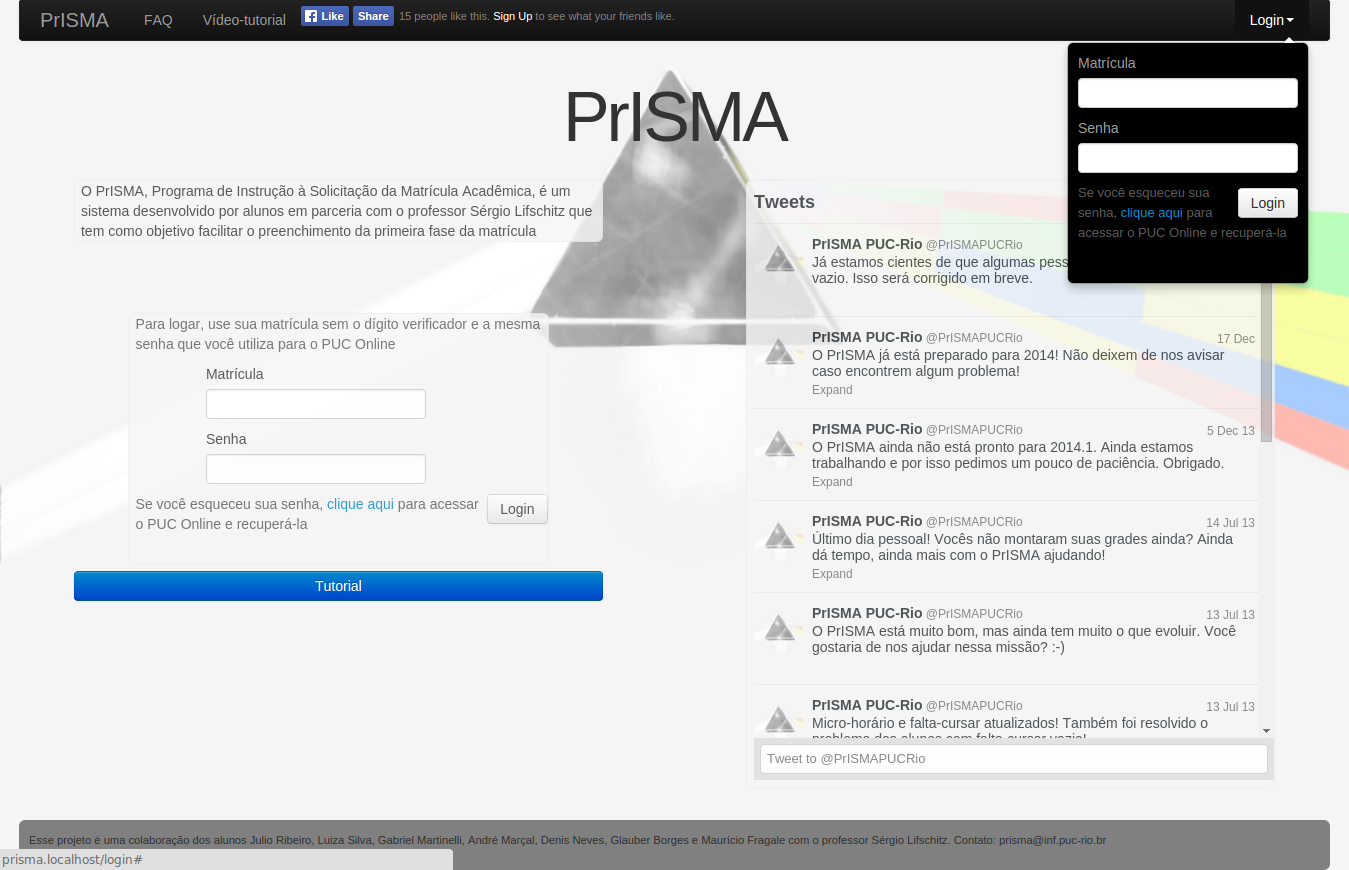
\includegraphics[width=0.9\linewidth]{img/v3_tela_login.png}
    \caption{Tela de login}
\end{figure}

Esta é a tela de entrada no sistema. Como pode ser visto, pode-se entrar por meio do formulário que é aberto ao clicar em "login", na barra superior. Da mesma forma, pode-se clicar em "fazer login", no meio da página, para se abrir o segundo formulário. Ambos tem comportamento idêntico. 

Nesta página também é possível notar a presença das notícias, que será explicado mais para frente.

\section{Termo de compromisso}

\begin{figure}[H]
    \centering
    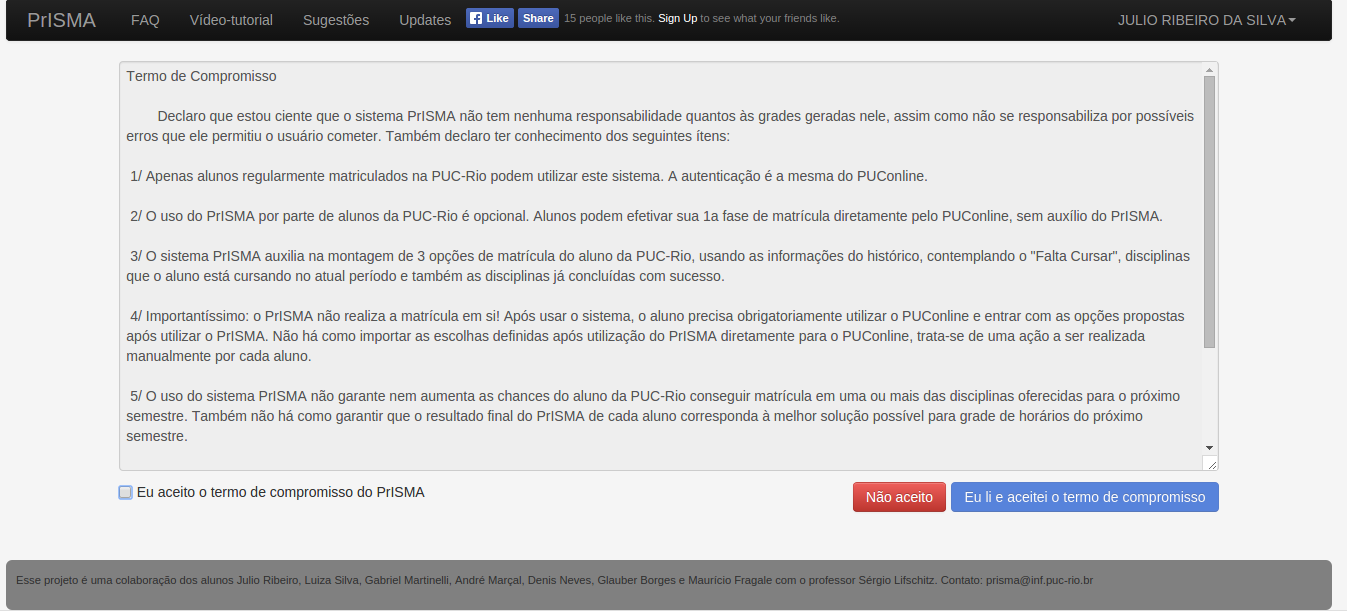
\includegraphics[width=\linewidth]{img/v3_tela_termo.png}
    \caption{Tela de termo de compromisso}
\end{figure}

Logo após realizar a entrada no sistema, caso seja a primeira vez ou o termo de compromisso ainda não tenha sido aceito, o sistema automaticamente encaminhará para a tela de termo de compromisso, conforme é apresentada acima. 

Esta tela é necessária para esclarecer ao aluno que o sistema se trata de um projeto acadêmico e não tem qualquer relação oficial com a PUC-Rio. O texto completo encontra-se abaixo:

\vspace{3 mm}

\textit{Termo de Compromisso}

\textit{Declaro que estou ciente que o sistema PrISMA não tem nenhuma responsabilidade quantos às grades geradas nele, assim como não se responsabiliza por possíveis erros que ele permitiu o usuário cometer. Também declaro ter conhecimento dos seguintes ítens:}

\textit{1/ Apenas alunos regularmente matriculados na PUC-Rio podem utilizar este sistema. A autenticação é a mesma do PUConline.} 

\textit{2/ O uso do PrISMA por parte de alunos da PUC-Rio é opcional. Alunos podem efetivar sua 1a fase de matrícula diretamente pelo PUConline, sem auxílio do PrISMA.}

\textit{3/ O sistema PrISMA auxilia na montagem de 3 opções de matrícula do aluno da PUC-Rio, usando as informações do histórico, contemplando o "Falta Cursar", disciplinas que o aluno está cursando no atual período e também as disciplinas já concluídas com sucesso.}

\textit{4/ Importantíssimo: o PrISMA não realiza a matrícula em si! Após usar o sistema, o aluno precisa obrigatoriamente utilizar o PUConline e entrar com as opções propostas após utilizar o PrISMA. Não há como importar as escolhas definidas após utilização do PrISMA diretamente para o PUConline, trata-se de uma ação a ser realizada manualmente por cada aluno.}

\textit{5/ O uso do sistema PrISMA não garante nem aumenta as chances do aluno da PUC-Rio conseguir matrícula em uma ou mais das disciplinas oferecidas para o próximo semestre. Também não há como garantir que o resultado final do PrISMA de cada aluno corresponda à melhor solução possível para grade de horários do próximo semestre.}

\textit{6/ Na versão atual, o PrISMA verifica pré-requisitos básicos e permite orientar o aluno para matrículas em disciplinas que ele PODE CURSAR. Assim, o aluno perceberá que para algumas disciplinas não é permitida a escolha para alguma opção - caso não tenha pré-requisitos, por exemplo - ou então há um aviso de atenção para disciplinas sendo cursadas, pois uma vez o aluno aprovado não poderá solicitar na matrícula, ou ainda, pode ser alguma disciplina pré-requisito de outra.}

\textit{7/ O PrISMA não garante que você está apto a cursar todas as turmas escolhidas. Isso ocorre pois as turmas podem ser destinadas a certos cursos e esse tipo de checagem não está sendo feita nessa versão.}

\vspace{3 mm}

Caso o termo de compromisso não seja aceito, não é permitido o prosseguimento na  utilização do sistema.

\section{Principal}

\begin{figure}[H]
    \centering
    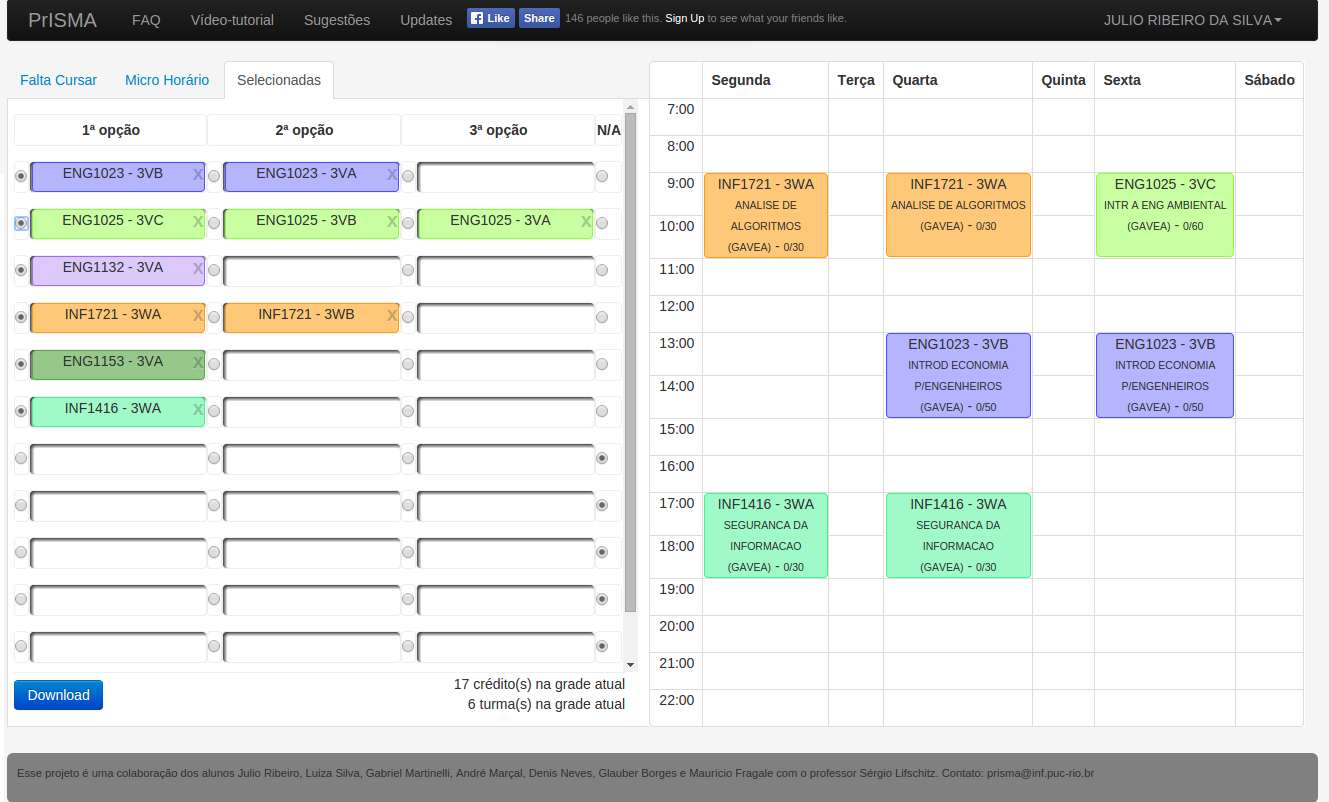
\includegraphics[width=0.85\linewidth]{img/v3_selecionadas.png}
    \caption{Tela principal do PrISMA}
\end{figure}

Uma vez que as credenciais foram corretamente verificadas e o termo de compromisso foi aceito, o sistema é redirecionado para a página principal do sistema. 

Nesta página existem muitas funcionalidades, conforme será explicado em mais detalhes nos próximos tópicos.

\subsection{Aba Falta-Cursar}

\begin{figure}[H]
    \centering
    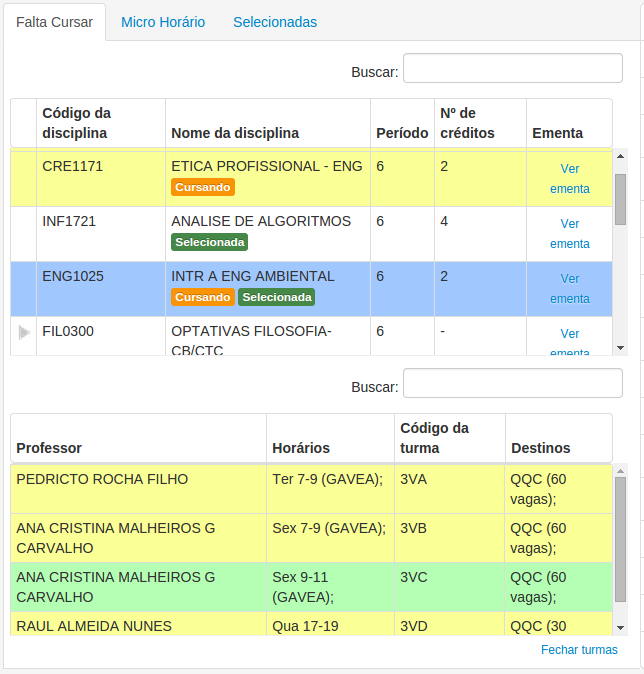
\includegraphics[width=0.7\linewidth]{img/v3_aba_falta_cursar.png}
    \caption{Aba Falta-Cursar}
\end{figure}

Nesta aba são apresentadas as disciplinas restantes que os alunos devem cursar. A tabela inferior apenas existe caso alguma disciplina na tabela superior tenha sido selecionada. E, como pode ser visto, existe um botão para fechar essa tabela de turmas. Vale notar que em ambas as tabelas existe um campo de busca, para o caso em que a quantidade de resultados é muito grande. Neste campo pode ser buscado pela informações contidas em quaisquer colunas das suas respectivas tabelas. 

Cada disciplina é apresentada por seu código e nome. O número de período associado se refere àquele sugerido pela universidade para se cumprir a disciplina. O número de créditos é um valor utilizado pela universidade para dar peso às disciplinas. O link da ementa redireciona para a página oficial da PUC-Rio, onde é apresentada a ementa, livros textos e pré-requisitos detalhados. 

Cada linha de disciplina pode apresenta três cores de fundo. São elas:

\begin{itemize}
	\item Vermelho: o aluno não cumpriu todos os pré-requisitos necessários para se cursar a disciplina. Neste caso, é desabilitado o clique e a sua lista de turmas não se abre. 
	\item Amarelo: informa para se tomar cuidado. Ou a disciplina está sendo cursada ou os pré-requisitos dependem de disciplinas que estão sendo cursadas para serem atendidos. Caso a disciplina esteja sendo cursada, uma marcação na cor caramelo é inserida ao lado do nome, informando este fato. 
	\item Branco: pré-requisitos foram validados e a disciplina pode ser cursada.
\end{itemize}

\begin{figure}[H]
    \centering
    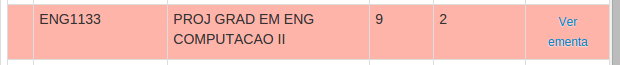
\includegraphics[width=0.7\linewidth]{img/v3_disciplina_presa.png}
    \caption{Disciplina presa por pré-requisito}
\end{figure}

Foi falado da marcação ao lado do nome da disciplina para demonstrar que ela está sendo cursada e, por isso, pode não ser necessário cursá-la no próximo período novamente. Da mesma maneira, quando alguma turma da disciplina é selecionada, é adicionada uma marcação na cor verde escuro informando que esta disciplina foi incluída no planejamento. 

Na tabela de turmas, que abre quando uma disciplina que pode ser cursada é selecionada, são apresentadas as turmas que serão disponibilizadas para o próximo semestre. A cor de fundo da linha também possui significado. Quando verde, informa que a turma foi selecionada. Em outros casos, significa que a turma não foi selecionada, e a cor exibida se refere à situação da disciplina, conforme foi apresentado anteriormente.  

Uma vez selecionada a turma, ela é automaticamente inserida na aba de selecionadas e, caso seu horário não conflite com o de nenhuma outra turma selecionada ou seja a primeira turma selecionada da sua respectiva disciplina, também é inserida automaticamente na tabela de horários.

\subsection{Aba Micro-Horário}

\begin{figure}[H]
    \centering
    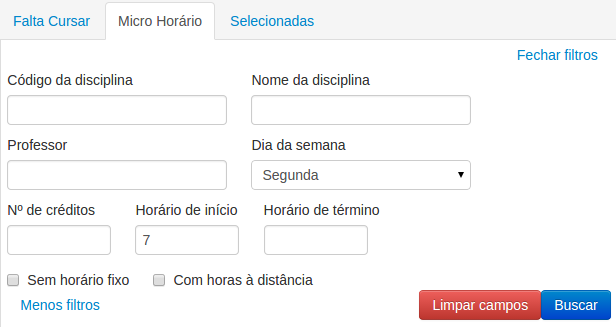
\includegraphics[width=0.8\linewidth]{img/v3_aba_microhorario.png}
    \caption{Aba Micro-Horário}
\end{figure}

Nesta aba pode-se busca por todas as turmas que serão oferecidas no próximo período. As turmas podem ser buscadas pelo seu código, nome, quantidade de créditos e horários, ou apenas parte destas informações. Ou seja, caso queira buscar pelas disciplinas do departamento de informática, que sabidamente possuem código que começam em "INF", basta colocar "INF" no campo de busca do código. Da mesma forma, nenhum campo é obrigatório. 

Uma vez realizada a busca, pode-se fechar os filtros completamente, clicando no botão localizado no canto superior direito. Pode-se limpar os campos de busca, para se realizar uma nova busca. Ou mesmo ocultar parte dos filtros clicando no botão "menos filtros".

\begin{figure}[H]
    \centering
    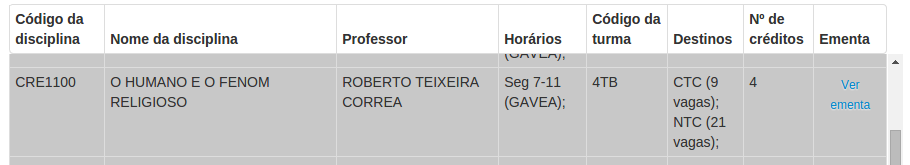
\includegraphics[width=0.8\linewidth]{img/v3_disciplina_cursada.png}
    \caption{Resultado da busca na aba Micro-Horário}
\end{figure}

A quantidade de colunas aqui apresentadas é maior do que na tabela de Falta-Cursar, por ter que apresentar os dados das disciplinas e turmas ao mesmo tempo. Nesta tabela a cor de fundo segue a mesma lógica de significado das tabelas do Falta-Cursar, tendo as cores branca, vermelha, amarela e verde. No entanto, a cor cinza foi adicionada para representar aquelas turmas cujas disciplinas já foram cursadas.

\subsection{Aba Selecionadas}

\begin{figure}[H]
    \centering
    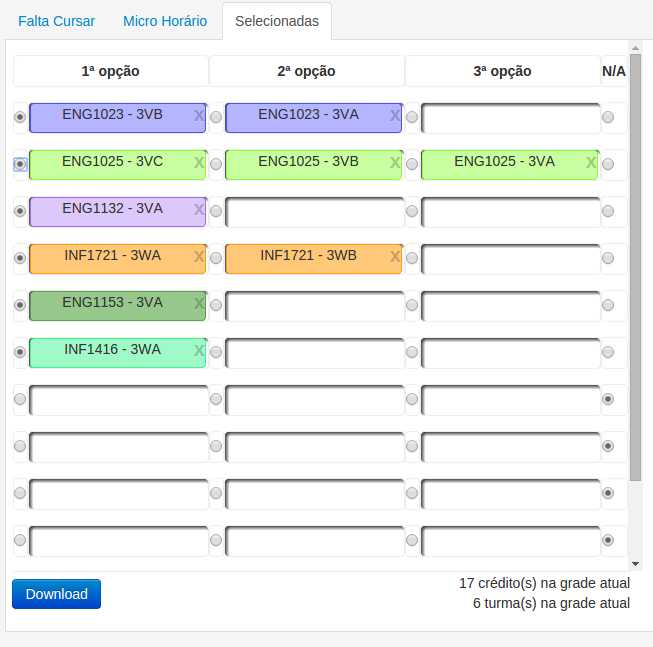
\includegraphics[width=0.8\linewidth]{img/v3_aba_selecionadas.png}
    \caption{Aba Selecionadas}
\end{figure}

Todas as turmas selecionadas na aba Falta-Cursar ou Micro-Horário são inseridas automaticamente nesta aba de selecionadas segundo os seguintes critérios: caso exista alguma outra turma da mesma disciplina da turma que está sendo inserida e, na sua respectiva linha existe opção não ocupada, insere na próxima opção disponível; caso contrário, insere em uma nova linha.  

Essa interface é baseada no sistema \textit{Solicitação de Matrícula}, explicado no capítulo 2. Foi feito dessa maneira para facilitar a transferência de dados entre os dois sistemas, de forma manual pelo aluno. No entanto, nesta mesma aba existe um botão de "download", que fornece um arquivo com todas as informações presentes nessa página para que, algum dia, seja possível ser importado automaticamente pela PUC-Rio. 

Nesta interface, é possível clicar e arrastar as turmas para que sejam trocadas de opção, ou mesmo linhas. Caso uma turma seja arrastada para cima de outra, elas trocam de posição. Da mesma forma, é possível arrastar as linhas para trocá-las de posição, modificando assim a prioridade das turmas nelas contidas. 

No lado esquerdo de cada turma existe um \textit{radio button}. Para cada linha apenas um pode ser selecionado, dado que apenas uma opção pode ser escolhida por linha. E caso nenhuma turma tenha sido selecionada em uma linha, aquele \textit{radio button} mais a direita que ficará selecionado.  

Define-se então a simulação de conflito de horários. O objetivo é simular exatamente o comportamento realizado pelo processamento feito no sistema \textit{Solicitação de Matrícula}. Isto é, as primeiras linhas e primeiras colunas tem prioridades e uma vez selecionada uma turma em uma linha, processa-se a próxima linha. 

Por exemplo, ao se clicar na turma que está na segunda opção da terceira linha, caso ela não conflita com nenhuma anteriormente selecionada, ela é selecionada e realiza a simulação para as linhas abaixo, ou seja, da quarta linha em diante. Vale ressaltar que, as segundas e terceiras opções das linhas mais acima tem prioridade em relação as primeiras opções das linhas mais abaixo. 

A quantidade de créditos totais e quantidades de turmas selecionadas na simulação é informada no canto inferior direito desta mesma aba. 

\subsection{Tabela de horários}

\begin{figure}[H]
    \centering
    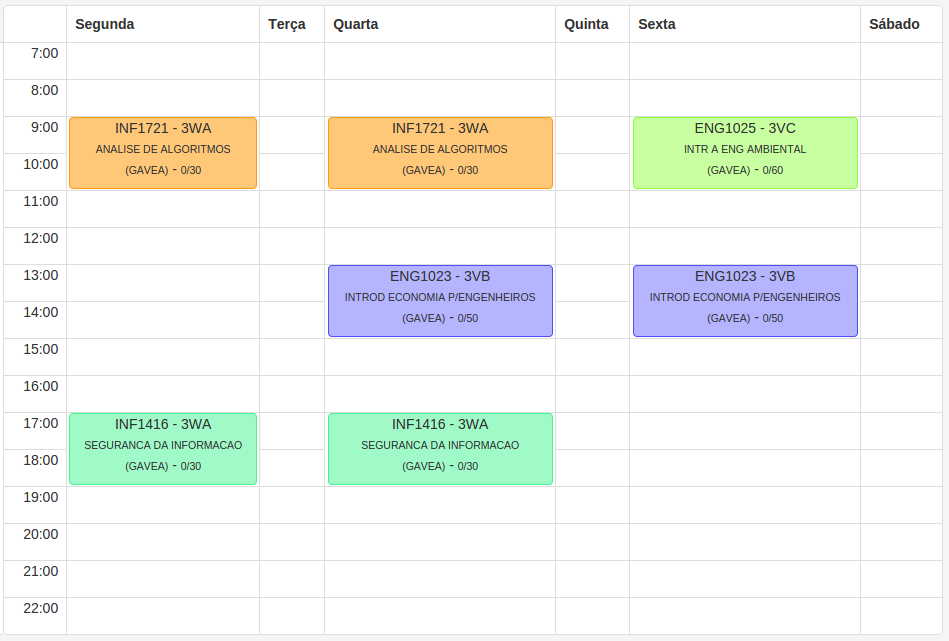
\includegraphics[width=\linewidth]{img/v3_tabela_horarios.png}
    \caption{Tabela de horários}
\end{figure}

A tabela de horários é visível durante toda a navegação pela página principal do PrISMA, ficando localizada no lado direito do sistema, ao contrário das abas que se encontram no lado esquerdo. 

O objetivo desta tabela de horários é oferecer uma fácil visualização do horário semanal que está sendo planejado. Em cada célula da tabela é possível a existência de apenas uma turma, por isso que a combinação de turmas apresentada é aquela resultado da simulação apresentada no tópico anterior, ao explicar a aba Selecionadas. 

Cada turma preenche todos os seus respectivos horários. A cor do bloco que representa cada turma está relacionada com a cor da linha que ela está inserida na aba Selecionadas, para melhor visualização. No bloco são informados código da disciplina, código da turma, nome da disciplina, localização do campus da universidade que ela será ministrada e uma informação de classificação do aluno segundo a quantidade de vagas. Esse último tem por objetivo informar a classificação do aluno em relação àqueles que também solicitaram essa turma, dentro do PrISMA. Dessa maneira, caso sua classificação seja maior que a quantidade de vagas, pode-se concluir que se trata de uma má escolha de turma. 

Essa tabela de horários se relaciona com a busca no Micro-Horário. Por exemplo, ao se clicar em uma célula vazia na tabela, o horário representado por esse célula será utilizado como parâmetro de busca no Micro-Horário, informando quais turmas podem preenchê-lo. Da mesma forma, ao se clicar sobre o bloco de alguma disciplina, será realizada a busca por todas as turmas da respectiva disciplina, facilitando a navegação pelas demais opções.

\section{Cabeçalho}

\begin{figure}[H]
    \centering
    
\includegraphics[width=\linewidth]{img/v3_header.png}
    \caption{Cabeçalho do sistema}
\end{figure}

No lado esquerdo do cabeçalho encontram-se os botões de FAQ, Video-tutorial, Sugestões e Updates, conforme será explicado mais para frente. Ao centro encontra-se o botão de "like" da rede social Facebook, de forma que o sistema seja mais facilmente divulgado. 

No lado direito, caso o usuário já esteja na parte interna do sistema, é exibido o seu nome. Ao clicar no seu nome, abre-se a opção de sair do sistema. Caso esteja na página de login, exibe-se um botão que, ao ser clicado, abre-se o formulário para entrada das credenciais de acesso ao sistema.

\subsection{Sugestões}

\begin{figure}[H]
    \centering
    
\includegraphics[width=0.7\linewidth]{img/v3_sugestoes.png}
    \caption{Interface de sugestões}
\end{figure}

Para aproximar o contato dos usuários do sistema com os desenvolvedores, foi disponibilizada essa interface para envio de sugestões e afins. Não existe limitação no tamanho do texto que pode ser enviado. 

Essa interface pode ser acessada ao clicar no botão Sugestões, presente no cabeçalho do sistema. Essa opção apenas é acessível quando as credenciais do usuário foram verificadas.

\subsection{Vídeo tutorial}

\begin{figure}[H]
    \centering
    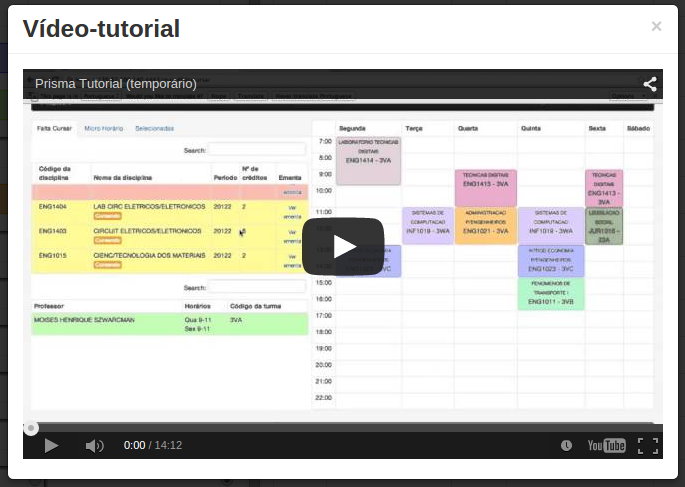
\includegraphics[width=0.7\linewidth]{img/v3_video_tutorial.png}
    \caption{Interface com o vídeo tutorial}
\end{figure}

Ao clicar no botão Video-tutorial, presente no cabeçalho, abre-se uma interface disponibilizando o vídeo tutorial. Neste vídeo\footnote{https://www.youtube.com/watch?v=XHF8WOJ6xI0} são explicadas todas as funcionalidades do sistema, de forma a auxiliar os alunos.

\subsection{FAQ}

\begin{figure}[H]
    \centering
    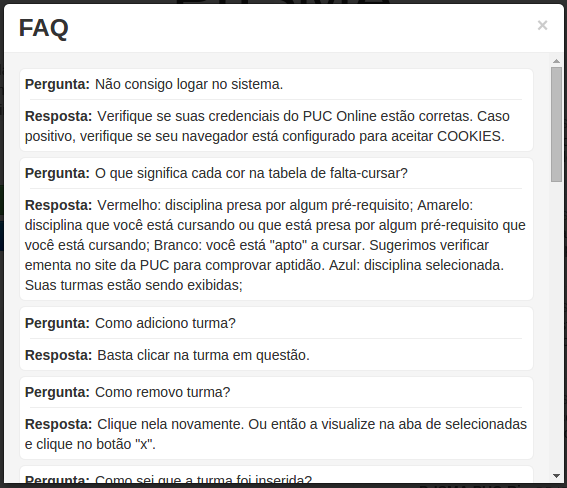
\includegraphics[width=0.7\linewidth]{img/v3_faq.png}
    \caption{Interface com as perguntas frequentes}
\end{figure}

Por se tratar de um sistema novo aos alunos, foi disponibilizada uma interface apresentando as dúvidas frequentes. 

Essas perguntas tem por objetivo responder dúvidas básicas. Para entendimento mais aprofundado quanto ao funcionamento da interface, recomenda-se a visualização do vídeo tutorial.

\newpage
\subsection{Conta no Twitter}

\begin{figure}[H]
    \centering
    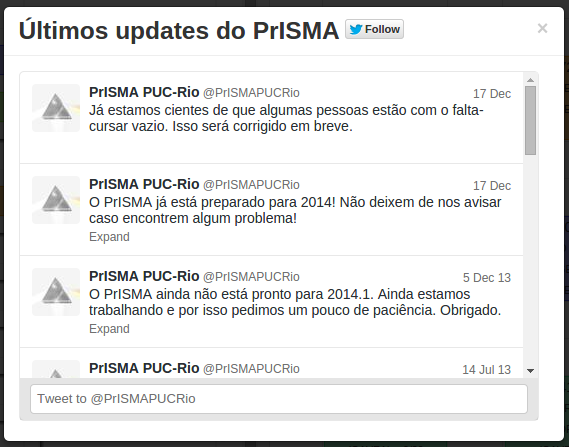
\includegraphics[width=0.6\linewidth]{img/v3_noticias.png}
    \caption{Interface com as notícias}
\end{figure}

Como forma de aproximar os desenvolvedores dos alunos que estavam fazendo uso do sistema, foi criada uma conta na rede social Twitter\footnote{https://twitter.com/prismapucrio} e integrada ao sistema. 

Ao contrário do campo de sugestões, pela rede social é possível responder dúvidas dos alunos, publicar notícias e divulgar o sistema.

\section{Estatísticas}

Como forma de auxiliar os administradores do sistema e aqueles que planejam a disponibilização das turmas para os próximos períodos, foram implementadas algumas estatísticas quanto à utilização do PrISMA, conforme será explicado. 

Todos os dados aqui apresentados se referem à utilização do sistema para o primeiro semestre de 2014, última vez que o PrISMA foi disponibilizado para os alunos da PUC-Rio.

\subsection{Total de alunos}

% \begin{figure}[H]
%     \centering
%     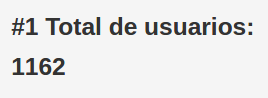
\includegraphics[width=0.4\linewidth]{img/v3_estatistica1.png}
%     \caption{Total de alunos}
% \end{figure}

Total de usuários que utilizaram o sistema em um período. Apenas um valor inteiro é apresentado.

\subsection{Acesso diário}

\begin{figure}[H]
    \centering
    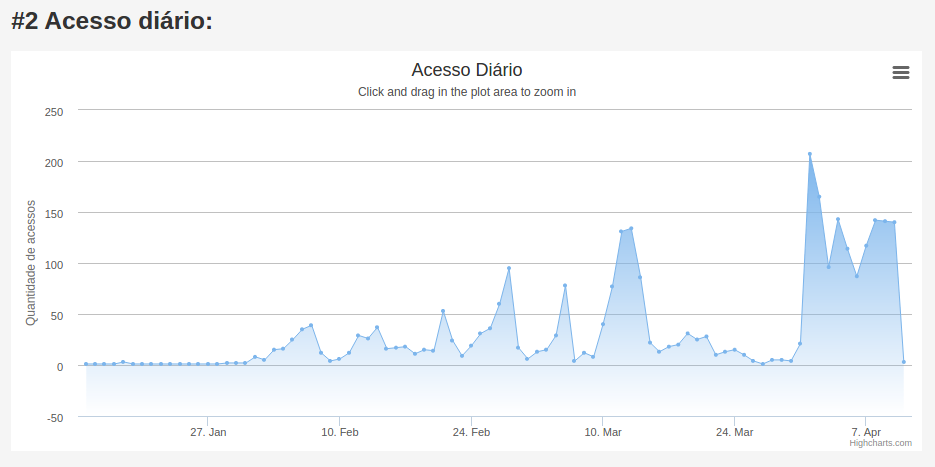
\includegraphics[width=\linewidth]{img/v3_estatistica2.png}
    \caption{Acesso diário}
\end{figure}

Gráfico que mostra a quantidade de alunos únicos que acessaram o sistema por dia. Como pode-se observar acima, a maior quantidade de acessos ao sistema ocorreu perto de acabar o prazo de solicitação de matrícula.

\subsection{Uso por curso}

\begin{figure}[H]
    \centering
    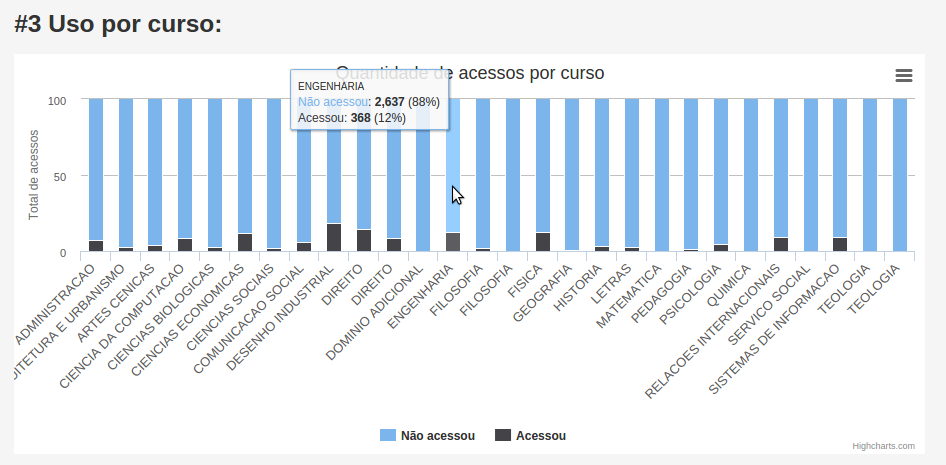
\includegraphics[width=\linewidth]{img/v3_estatistica3.png}
    \caption{Uso por cuso}
\end{figure}

Informa a porcentagem de utilização dos alunos, filtrado por seus cursos. Ao passar o mouse em cima de cada curso, mostra-se a quantidade total de alunos do respectivo curso e quantos deles acessaram o PrISMA.

\subsection{Demanda por turma}

\begin{figure}[H]
    \centering
    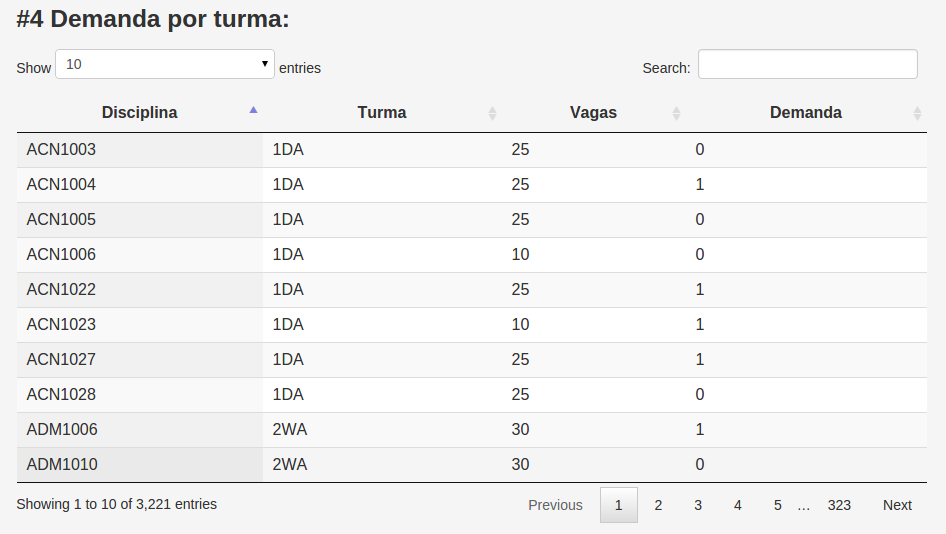
\includegraphics[width=0.7\linewidth]{img/v3_estatistica4.png}
    \caption{Demanda por turma}
\end{figure}

Para cada turma oferecida para o próximo período, informa a demanda de alunos e a quantidade de vagas. Pode-se filtrar pelo nome da disciplina e código da turma. 

Esta funcionalidade serve de base para os coordenadores de departamentos avaliarem a necessidade ajustes no planejamento das turmas.


\chapter{Resultado}

Antes do desenvolvimento desta versão documentada, a versão antiga do PrISMA já havia sido disponibilizada para os alunos da PUC-Rio durante dois anos. Isto é, desde o início do ano de 2011 até o final do ano de 2012. Nesse período o sistema foi acessado por 300 alunos, em média, por período. Esse número não é tão representativo por causa da divulgação, que foi feita apenas para o Departamento de Informática da PUC-Rio. 

Para esta nova versão, no entanto, a divulgação foi feita para toda a PUC. Ela começou a ser disponibilizada no início do ano de 2013 até o início do ano de 2014, representando assim três períodos. No primeiro período, 1490 alunos utilizaram o sistema. No segundo, foram 2093 e, no último, 1162 alunos. Esse aumento na quantidade de acessos é justificado pelo apoio na divulgação por parte do professor Washington Braga. 

Quanto aos requisitos funcionais, todos foram atendidos. O resultado final atendeu a todas as expectativas. Seguem alguns feedbacks deixados pelos alunos na seção de sugestões:

\vspace{3 mm}

\textit{2013-01-08 23:07h - Boa noite, primeiramente gostaria de parabenizar pelos avanços que tem sido feitos no prisma. A sugestão que gostaria de dar para vocês é a de colocar uma opção que permita arquivar/salvar até 2 ou 3 grades feitas e assim o aluno possa compará-las com mais eficiência e agilidade. O motivo para isso é porque, as vezes, pensamos em por eletivas ou até matérias do próprio currículo diferentes ou em outros horários para ver qual seria a que mais lhe agradaria. Não é algo fundamental mas seria de grande ajuda. Obs: Se fosse possível eu obter um retorno sobre isso ficaria muito grato. Obrigado , Matheus}

\vspace{3 mm}

\textit{2013-07-10 00:29h - Gostaria de agradecer pelo excelente sistema e dizer que ele foi primordial para fazer a minha grade horária. Muito Obrigado.}

\vspace{3 mm}


\chapter{Trabalhos futuros}

Apesar do sucesso do sistema, algumas funcionalidades ainda podem ser adicionadas. A primeira delas é a integração oficial com o sistema do PUC Online, de forma que o aluno não precise se planejar em um ambiente, e entrar com os dados oficialmente em outro.

Atualmente, para cada período novo, alguns cuidados devem ser tomados na hora de importar os dados. Se faz necessário a criação de uma página de administrador, onde seria possível avaliar todo o comportamento do sistema, assim como inserir e remover usuários que não sejam alunos.

As estatísticas estão devidamente implementadas, mas poderiam ser melhor direcionadas para quem está visualizando. Neste caso, deveria haver conta de coordenador de departamento, que teria acesso à todos os dados referentes aos seus cursos.

Deveria ser possível adicionar e remover turmas diretamente no PrISMA, enquanto está sendo utilizado pelos alunos. Essa necessidade aparece naturalmente ao visualizar as estatísticas e constatar que a oferta de turmas não condiz com a demanda.

No mesmo contexto do problema dos alunos, diversas ferramentas poderiam ser utilizadas para auxiliar o coordenador na hora de organizar as turmas a serem oferecidas. Também poderia haver um mapeamento de salas e disponibilidades de professores, assim como as disciplinas que podem ser ministradas por eles.

E, para finalizar, resolver pequenos problemas de implementação e refinar as funcionalidades já implementadas.

%%%%%%%%%%%%%%%%%%%%%%%%%%%%%%%%%%%%%%%%%%%%%%%%%%%%%%%%%%%%%%%%%%%%%%%%%%%%%%%%
\arial
\nocite{*}
\bibliography{relatorio2}

\normalfont

\appendix

\chapter{Principais trexos de códido do Banco de Dados}

\section{Função AlunoDisciplinaApto}

\begin{figure}[H]
    \centering
    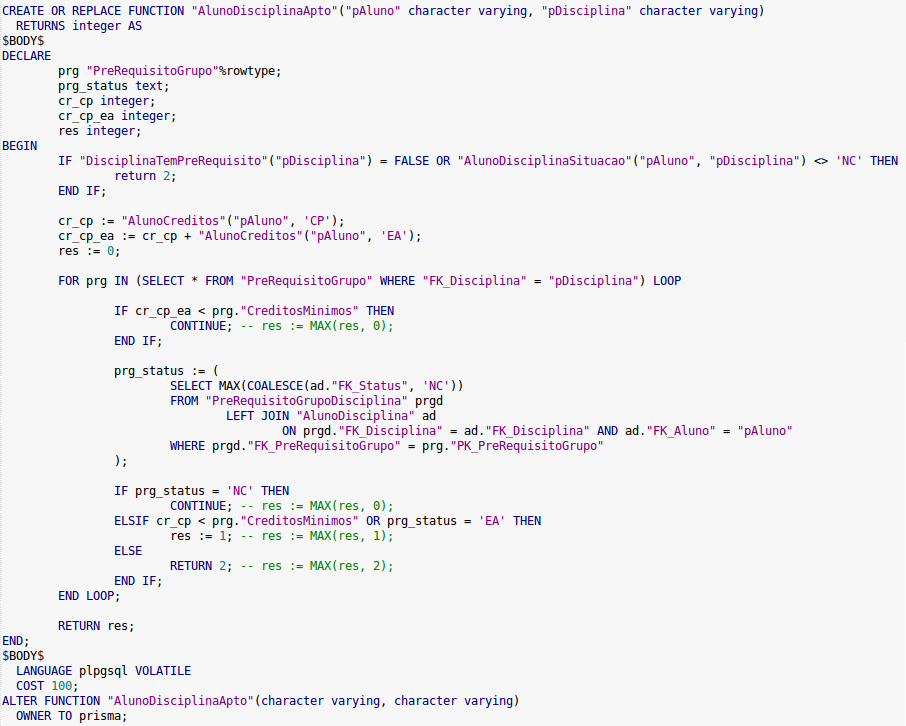
\includegraphics[width=\linewidth]{img/v3_func_alunoapto.png}
    \caption{Função AlunoDisciplinaApto}
\end{figure}

\section{Função AlunoCreditosCursados}

\begin{figure}[H]
    \centering
    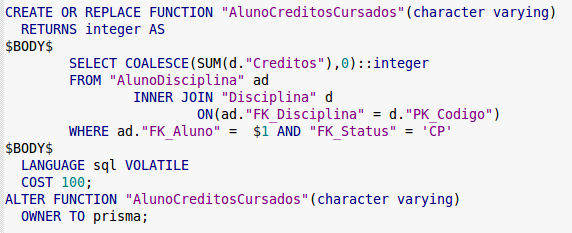
\includegraphics[width=0.7\linewidth]{img/v3_func_alunocreditoscursados.png}
    \caption{Função AlunoCreditosCursados}
\end{figure}

\section{Função AlunoTurmaRank}

\begin{figure}[H]
    \centering
    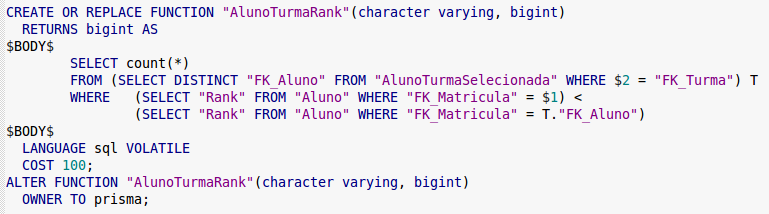
\includegraphics[width=0.9\linewidth]{img/v3_func_alunorank.png}
    \caption{Função AlunoTurmaRank}
\end{figure}


\section{Função AlunoDisciplinaSituacao}

\begin{figure}[H]
    \centering
    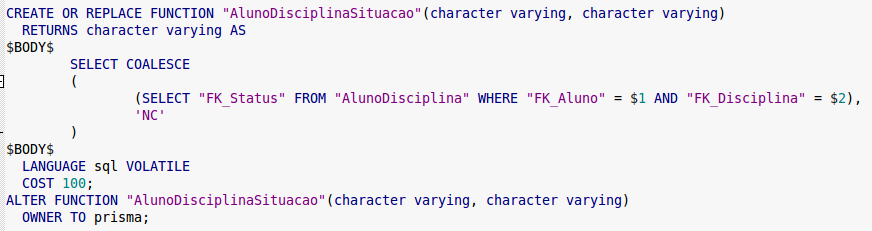
\includegraphics[width=\linewidth]{img/v3_func_alunosituacao.png}
    \caption{Função AlunoDisciplinaSituacao}
\end{figure}

\section{Função DisciplinaTemPreRequisito}

\begin{figure}[H]
    \centering
    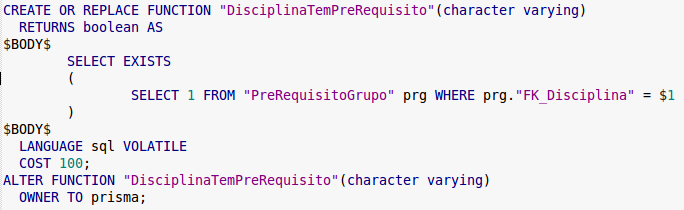
\includegraphics[width=0.9\linewidth]{img/v3_func_discplinaprerequisito.png}
    \caption{Função DisciplinaTemPreRequisito}
\end{figure}

\section{Função AlunoOptativaCursada}

\begin{figure}[H]
    \centering
    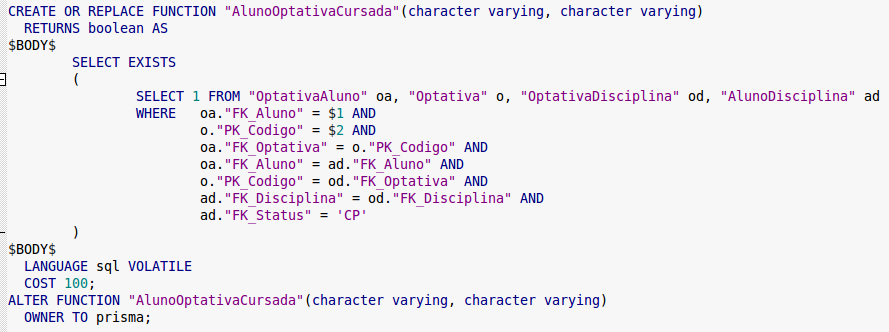
\includegraphics[width=\linewidth]{img/v3_func_optativacursada.png}
    \caption{Função AlunoOptativaCursada}
\end{figure}



\chapter{Análise de complexidade}

Nesta seção será discutido sobre a complexidade do problema de decisão trabalhado pelo PrISMA. Este artigo foi escrito pela Luiza de Noronha, orientada pelo professor Sérgio Lifschitz.

\section{Definição do problema}

(...) podemos especificar com mais precisão o problema geral que deve ser resolvido:

\vspace{3 mm}
\textit{Dada uma lista L de turmas e um conjunto M de matérias que o aluno deseja cursar, busca-se retornar uma grade de disciplinas e horários para o aluno válida que utiliza um subconjunto de M com a maior cardinalidade possível.}
\vspace{3 mm}

\section{Versão do problema de decisão}

A primeira concepção, que deu origem ao sistema PrISMA, era a versão de decisão do problema de otimização apresentado anteriormente, ou seja, dado um grupo de matérias, ela retornava uma solução que envolvia todas as matérias selecionadas pelo aluno ou dizer que não era possível combinar todas. Mais precisamente:

\vspace{3 mm}
\textit{Dada a lista de turmas disponíveis para cada matéria T e uma lista de matérias distintas L, gostaríamos de saber se é possível formar uma grade escolhendo exatamente uma turma ofertada para cada matéria em L.}
\vspace{3 mm}

Dado um conjunto de turmas P, é possível conferir se P é solução para nosso problema da seguinte forma:

\begin{itemize}
	\item Primeiramente é preciso verificar se todas as matérias das turmas escolhidas são distintas, o que pode ser feito com um algoritmo O($|P|^2$) simples, comparando cada matéria com todas as outras;
	\item Em seguida, é necessário checar se nenhum horário colide em P, o que também pode ser feito par a par com um algoritmo O($|P|^2$);
	\item Uma vez de posse de uma possível grade, basta verificar se trata-se de uma grade que contém todas as matérias da lista L, o que pode ser feito em O($|P|*|L|$), fazendo comparações par a par entre L e P;
\end{itemize}

Com todos os passos da verificação da solução resolvidos em tempo polinomial,possível conjecturar que nosso problema na prática pertence à classe NP.

A primeira observação trivial para esse problema é que não é necessário considerar as turmas das matérias (ou disciplinas) que não estão na lista L. Além disso, também é útil separar as turmas por matéria pois, segundo as restrições dadas, precisaremos pegar exatamente um elemento de cada conjunto.

A solução exponencial que segue é bastante natural: escolha uma turma qualquer da primeira matéria e tente todas as soluções possíveis que a incluam na grade. Se nenhuma solução for válida, tente a próxima matéria, até terminar o conjunto. Se isso acontecer, a resposta para nosso problema de decisão é não, caso contrário, sim.

Encontrar todas as soluções incluindo uma turma específica é o mesmo que resolver o problema para o conjunto sem considerar essa turma, mas verificando se as turmas inseridas não colidem com as turmas já selecionadas pelo algoritmo para montar a grade. Cabe observar que uma solução vazia, caso base dessa recursão, é sempre válida. A prova de correção desta solução é imediata também já que, no pior caso, ela tenta todas as possibilidades do conjunto de possíveis soluções.

\begin{figure}[H]
    \centering
    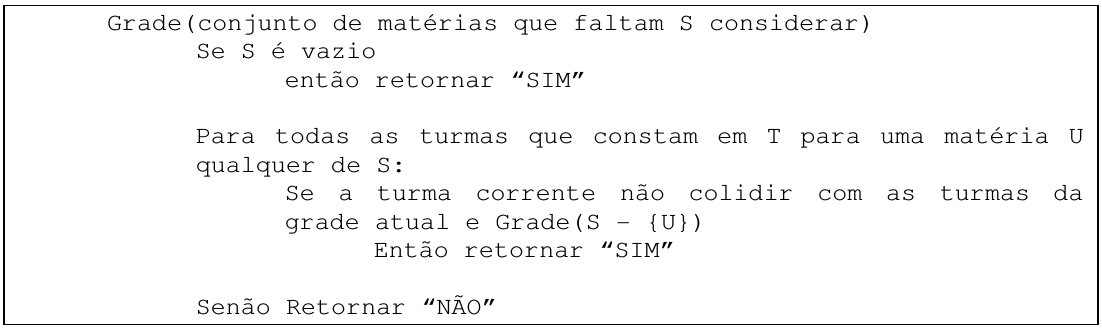
\includegraphics[width=\linewidth]{img/algoritmo_grade.png}
    \caption{Solução exponencial.}
\end{figure}

Notar que essa solução, por testar todas as possibilidades, tem complexidade igual ao produtório do número de turmas de cada matéria da lista, o que faz com seja potencialmente pouco eficiente se a lista for muito grande ou uma matéria tiver muitas possibilidades de turmas.

Uma pequena otimização que melhora bastante o caso médio do algoritmo é ordenar as matérias pelo número de turmas, em ordem ascendente. Isso diminui o branching factor do algoritmo, mas não diminui a complexidade. Cabe observar que, mesmo assim, a versão implementada (no caso, foi feito em JavaScript), tinha boa performance média na prática, para as solicitações de alunos testadas.

\section{Versão do problema de otimização}

Com o sistema já em produção e sendo utilizado pelos alunos da PUC-Rio, foi decidido que a abordagem de solução do problema deveria ser mudada. Ao invés de retornar uma grade com todas as matérias, o objetivo deveria ser retornar uma grade que maximizasse o número de matérias utilizadas na grade final. Reformulando:

\vspace{3 mm}
\textit{Dada a lista de turmas disponíveis para cada matéria T e uma lista de matérias distintas L, montar uma grade máxima, ou seja, uma grade tenha o maior número de matérias possível.}
\vspace{3 mm}

É imediato perceber que, para essa abordagem, sempre existirá uma grade não-vazia se alguma das matérias em L tiver pelo menos uma turma em T, já que com apenas uma turma não há colisões.

A partir do algoritmo discutido anteriormente para a solução do problema de decisão para um determinado conjunto de matérias, é possível considerar um algoritmo que, para cada um dos subconjuntos da lista de matérias L, execute o algoritmo anterior guardando-se o subconjunto máximo para o qual o algoritmo respondeu "SIM".

Uma maneira de otimizar o tempo médio do algoritmo e simplificar a implementação é começar com o conjunto completo, para em seguida considerar todos os conjuntos que têm um elemento a menos. Isso permite que uma vez o algoritmo tenha respondido “SIM” para algum conjunto, o processo possa ser finalizado, já todas as possibilidades melhores que aquele conjunto já foram testadas.

\begin{figure}[H]
    \centering
    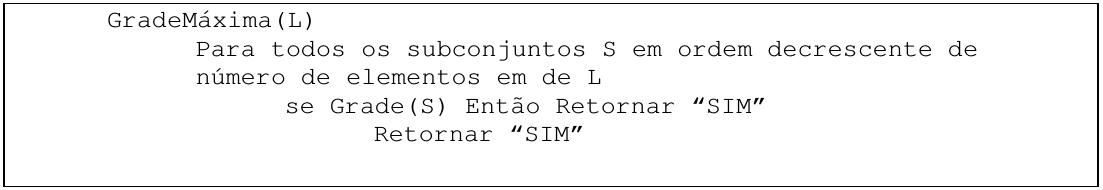
\includegraphics[width=\linewidth]{img/algoritmo_grade_maxima.png}
    \caption{Solução alternativa.}
\end{figure}

Esse algoritmo é mencionado aqui por questão de completitude, já que ele multiplica a complexidade do algoritmo anterior, que já era alta, pelo número de subconjuntos do conjunto das matérias, tornando-o impraticável. Assim, podemos reformular uma vez mais nosso problema:

\vspace{3 mm}
\textit{Dada a lista de turmas disponíveis no período de interesse L e o conjunto de matérias que o aluno deseja fazer T, é possível fazer uma lista S que contém somente turmas listadas em L de matérias contidas em T.}
\vspace{3 mm}

A partir da lista de turmas S, podemos montar um grafo da seguinte forma: cada turma é representada por um vértice e turmas incompatíveis têm arestas entre si – lembrando que turmas incompatíveis são turmas da mesma matéria cujos horários conflitam.:

\begin{figure}[H]
    \centering
    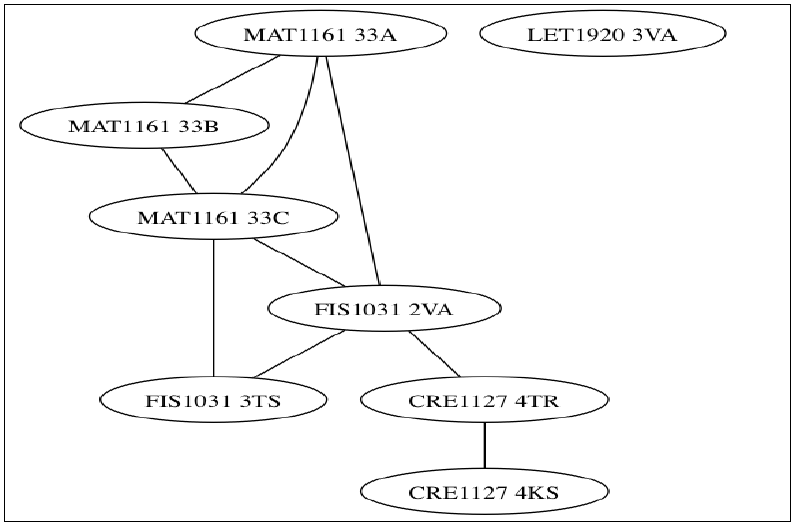
\includegraphics[width=\linewidth]{img/independentset.png}
    \caption{Grafo de incompatibilidades.}
\end{figure}

Este grafo foi gerado tomando como exemplo os seguintes códigos de disciplinas (MAT1161, FIS1031, CRE1127 e LET1920) e as turmas respectivas, ilustrado a seguir:

\begin{itemize}
	\item MAT1161:
	\begin{itemize}
		\item 33A: seg 13-15, qua 13-15
		\item 33B: seg 11-13, ter 15-17
		\item 33C: seg 7-9, qui 9-11
	\end{itemize}

	\item FIS1031:
	\begin{itemize}
		\item 2VA: seg 13-15, qui 9-11
		\item 3TS: seg 7-9, qua 7-9
	\end{itemize}

	\item CRE1127:
	\begin{itemize}
		\item 4TR: ter 9-11, qui 9-11
		\item 4KS: seg 15-17, qua 15-17
	\end{itemize}

	\item LET1920:
	\begin{itemize}
		\item 3VA: sex 9-11
	\end{itemize}
\end{itemize}

Podemos observar de imediato que todo conjunto independente desse grafo é uma grade válida. Então, nosso problema na verdade é reduzido para um \textit{Maximum Independent Set}, onde o número de nós é $|S|$. O algoritmo trivial para o \textit{Maximum Independent Set} é $\Omega((n^2)*(2^n))$, onde são examinados todos os subconjuntos de vértices e, para cada um desses subconjuntos, conferimos se corresponde a um conjunto independente.

Como o Maximum Independent Set é um problema clássico, existe uma série de algoritmos mais eficiente, como por exemplo aquele proposto em [4]\footnote{J.M. .Robson, “Algorithms for maximum independent sets", Journal of Algorithms 7 (3): pp 425–440, 1986} que tem complexidade assintótica O($2^{(0.276*n)}$). Entretanto, são muito mais complicados de implementar porque usam técnicas com distinções em muitos casos.

Por isso, optamos para a primeira versão: utilizar uma heurística, que pode garantir ao menos uma resposta não-vazia, mas não necessariamente a máxima. Essa \textit{Heurística de Grade Maximal} é uma variação do algoritmo usado no problema de decisão, onde tentamos cada turma para uma matéria e, se não for possível montar uma grade com nenhuma dessas turmas, tentamos construir uma resposta excluindo aquela matéria.

\begin{figure}[H]
    \centering
    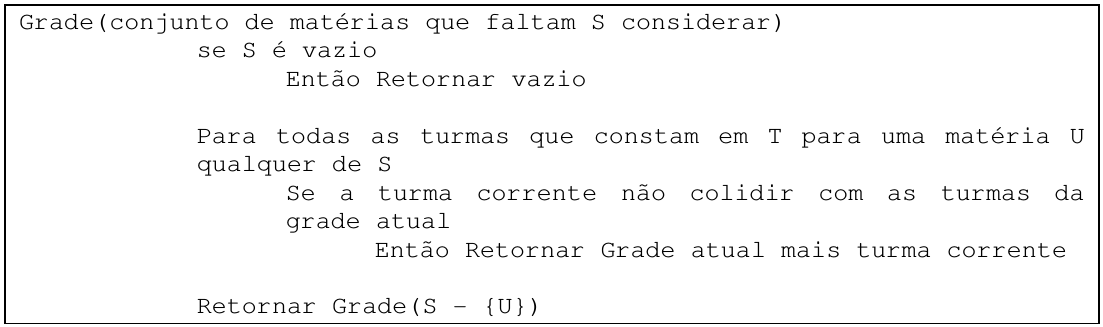
\includegraphics[width=\linewidth]{img/algoritmo_grade_maximal.png}
    \caption{Heurística de grade maximal.}
\end{figure}

Essa heurística garante uma grade que não pode ser expandida com a adição de nenhuma turma das disciplina que interessam ao aluno, mas pode retornar uma grade com apenas uma disciplina se a primeira delas colidir com todas as demais turmas de todas as outras disciplinas.

No caso, é possível ver que a grade gerada é maximal porque antes de ser testada a possibilidade de não incluir a matéria na grade, todas as turmas dessa matéria são testadas. Assim, se alguma das alternativas gerasse uma grade válida, já teria sido gerada uma solução usando essa turma.

\end{document}
